\documentclass[12pt]{article}

\usepackage{graphicx}
\usepackage{amsmath}
\usepackage{amssymb}
\usepackage{multicol}
\usepackage{multicap}
\usepackage{subfig}
\usepackage{scicite}

\renewcommand\refname{References}

\usepackage{geometry}
\geometry{left=3cm,right=3cm,top=2cm,bottom=2cm}

\usepackage{indentfirst}
\setlength{\parindent}{0em}

\newcounter{lastnote}
\newenvironment{scilastnote}{%
\setcounter{lastnote}{\value{enumiv}}%
\addtocounter{lastnote}{+1}%
\begin{list}%
{\arabic{lastnote}.}
{\setlength{\leftmargin}{.22in}}
{\setlength{\labelsep}{.5em}}}
{\end{list}}

\title{Supplement Material:\\ An Investigation on How Dynamics of macromolecules Influence Their Assembly Units with a Data-driven Approach}

\author
{Wangfei Yang,$^{1,2}$ Lorenzo Boninsegna,$^{1,3}$ Wenwei Zheng$^{4}$\\ and Cecilia Clementi$^{1,3\ast}$\\
\\
\normalsize{$^{1}$Center for Theoretical Biological Physics, Rice University, Houston, TX, USA}\\
%\normalsize{Houston, TX 77005, USA}\\
\normalsize{$^{2}$Systems, Synthetic and Physical Biology Program, Rice University, Houston, TX, USA}\\
%\normalsize{6100 Main St. Houston, TX 77005, USA}\\
\normalsize{$^{3}$Department of Chemistry, Rice University, Houston, TX, USA}\\
\normalsize{$^{4}$College of Integrative Sciences and Arts, Arizona State University, Mesa, AZ, USA}\\
\\
\normalsize{$^\ast$To whom correspondence should be addressed; E-mail:  cecilia@rice.edu.}
}

\date{\today}

\begin{document}

\maketitle

\section*{S3D Work Flow Summary}

The original paper of S3D algorithm has provided the entire work flow in detail\cite{Lrenzo_S3D}. But just for convenience, here a brief summary of this algorithm is provided as follow:

\ \ 

\hangindent=0.7cm
1. Given sources of data {\it i.e.} the trajectories of long-equilibrium all-atom simulations, we first use {\it Time-lagged Independent Component Analysis} (TICA) to obtain a subspace with reduced dimension that preserves the long-timescale dynamics of the system\cite{TICA}. TICA is analogous to {\it Principal component analysis}, but instead of considering the directions of largest variation, it considers the directions of slowest motions. We denote the input data (not just Cartesian coordinates but also features such as backbone torsions and residue pairwise distances that are extracted form the all-atom trajectory) as ${\bf X}_{T, n}$, where T is the length of the trajectory and n is the number of features. Then we choose a lag-time, which defines the temporal shift of correlations:
\begin{equation}
{\bf X}_{0} = \begin{pmatrix}
x_{1,1} & \cdots\ & x_{1,n} \\
\vdots & & \vdots \\
x_{T-\tau,1} & \cdots\ & x_{T-\tau,n}\\
\end{pmatrix} \ \ 
{\bf X}_{\tau} = \begin{pmatrix}
x_{\tau,1} & \cdots\ & x_{\tau,n} \\
\vdots & & \vdots \\
x_{T,1} & \cdots\ & x_{T,n}\\
\end{pmatrix}
\end{equation}
Then we calculate the correlation matrices:
\begin{equation}
{\bf C}_{00} = {\bf X}_{0}^{T}{\bf X}_{0} \ \ \ \ 
{\bf C}_{0\tau} = {\bf X}_{\tau}^{T}{\bf X}_{0}
\end{equation}
By solving the generalized eigenvalue problem:
\begin{equation}
{\bf C}_{0\tau}{\bf R} = {\bf C}_{00}{\bf R}{\bf \Lambda}
\end{equation}
where $R$ is the eigenvector matrix, and $\Lambda$ is the diagonal matrix of eigenvalues, we can project the trajectory onto the first several TICA eigenvectors so that we can obtain a set of lower-dimensional data which we call TICA coordinates\cite{variational_approach,variational_principle}.

\hangindent=0.7cm
2. Then, we use k-means clustering to discretize the phase space (here the one spanned by the TICA eigenvectors we chose in step 1) by assigning the configurations of each time steps into different discrete states\cite{TICA_collective_variable,TICA_commute_map}. Next, we obtain the discrete trajectory as one discrete state index for each time step. Then, we build a Markov state model (MSM) upon the discrete trajectory by counting the transitions between the discrete states\cite{MSM}.

\hangindent=0.7cm
3. On the top of the MSM, we then extract the coarse-grained kinetic model to identify the metastable states (such as folded, unfolded, or intermediate state) using Hidden Markov Model (HMM) estimation. By calculating the implied timescales from the transition matrix of the MSM, we can have some sense on how many metastable states there are. After this, we build a HMM which is defined by its transition matrix ${\bf T}(\tau)$ and a membership matrix ${\bf M}_{M,K}$\cite{HMM}, where M is the number of the discrete states and K is the number of the hidden states found by maximizing the likelihood of the HMM associated with the discrete trajectory ${\bf S}_{T}$:
\begin{equation}
{\bf P}({\bf S}_{T}| {\bf T}(\tau),{\bf M}_{M,K})
\end{equation}

\hangindent=0.7cm
4. After the state space is decomposed, we then perform decomposition on the structure. Here the method we use is called space time diffusion map\cite{Lrenzo_S3D,diffusion_map,diffusion_map_clustering}, with which  we can obtain the coherent domains, {\it i.e.} groups of atoms that preserve their geometric integrity under time evolution. Let ${\bf x}_{i,t} \in {\mathbb R}^{3}$ denote the position of atom i at time step t. We define the similarity matrix ${\bf W}_{t}$ of the diffusion map as:
\begin{equation}
{\bf W}_{t,ij} = exp(- \frac{||{\bf x}_{i,t}-{\bf x}_{j,t}||^{2}}{\epsilon})
\end{equation}
where $||\cdot||$ is Euclidean distance, and $\epsilon$ is a scale parameter. Then within each metastable state, we average the similarity matrices of different time steps to obtain a time-averaged similarity matrix to conduct clustering on the structure. At last, assembly units are obtained as the intersections of the coherent domains from different metastable states.

\section*{Coherent Domains of Each Metastable State for 10 Fast-folding Proteins}

\setlength{\parindent}{2em}

The details of metastable states identification and the coherent domains of each state obtained with Space Time Diffusion Map for the 10 fast-folding proteins are provided in fig-\ref{CLN025} to fig-\ref{lambda}. For each metastable state, we plot the representative structure, which obtained by first sampling then picking the one has the minimal average RMSD with all others, on the left with different coherent domains shown in different colors. And on the right, we plot the coherent domains linearly along the heavy atom sequence, similarly, using different colors to indicate different coherent domains. Moreover, there's one fact need to be noted that the coherent domains can be discontinuous, because it is possible that in some compact conformation 2 segments of the molecule will always stay together even though they are not sequentially close. The simulation details of these 10 fast-folding proteins can be found in reference \cite{A3D_frustration}.

\subsection*{Chignolin}

\begin{figure}[htbp]
  \centering
  \subfloat[Metastable State 1]{
  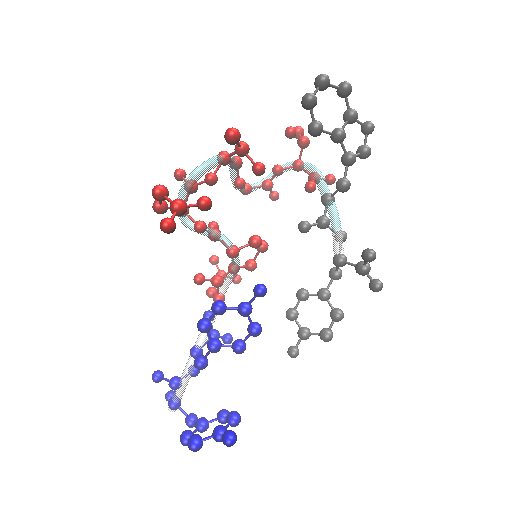
\includegraphics[width=0.3\textwidth, trim={0cm 0cm 0cm 0cm},clip]{CLN025_state_0.png}
  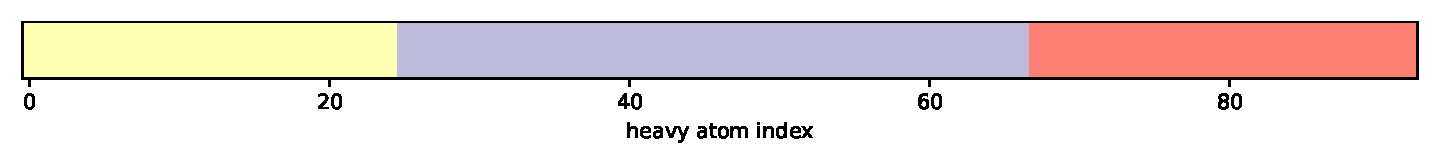
\includegraphics[width=0.7\textwidth]{CLN025_clustering_result_state_1.pdf}}\\
  \subfloat[Metastable State 2]{
  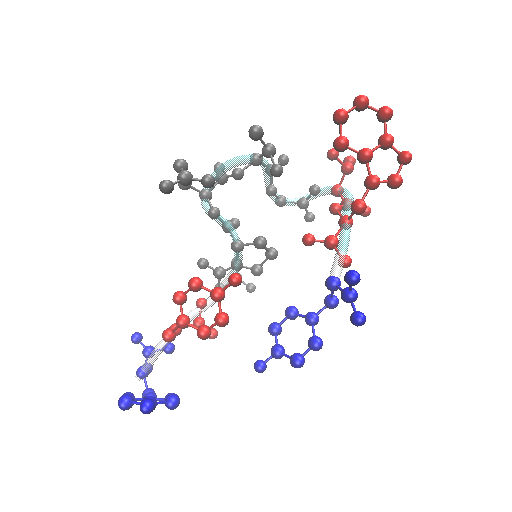
\includegraphics[width=0.3\textwidth, trim={0cm 0cm 0cm 0cm},clip]{CLN025_state_1.png}
  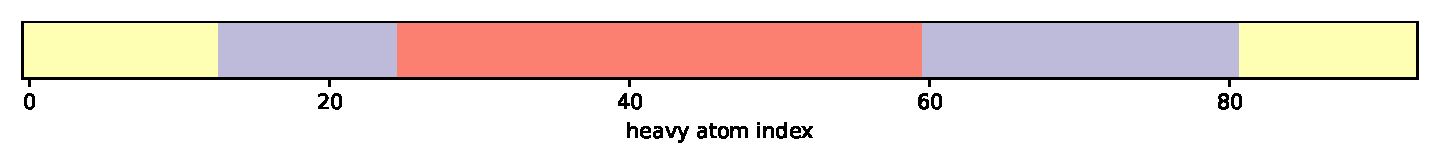
\includegraphics[width=0.7\textwidth]{CLN025_clustering_result_state_2.pdf}}\\
  \caption{\label{CLN025}Coherent domains for each metastable state of Chignolin. Two metastable states are identified. Three coherent domains are obtained for each state.}
\end{figure}

\clearpage

\subsection*{Trp-cage}

\begin{figure}[htbp]
  \centering
  \subfloat[Metastable State 1]{
  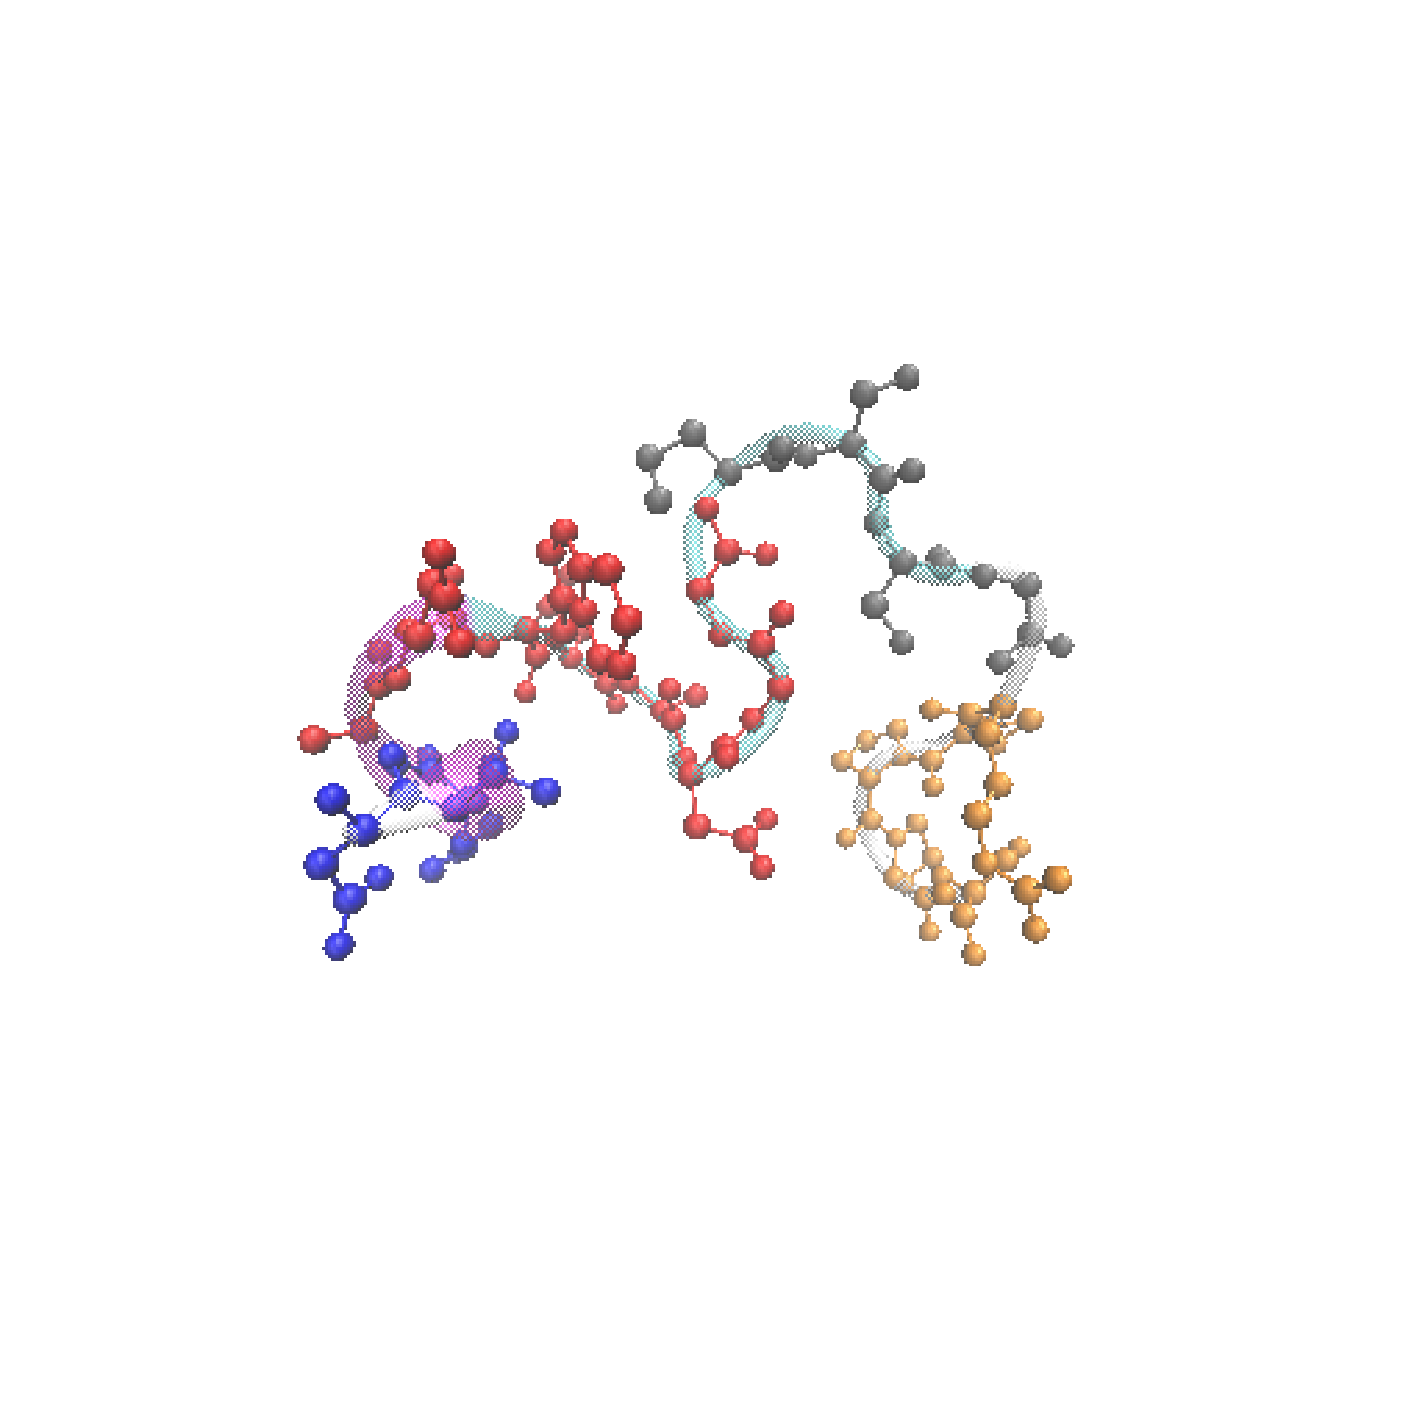
\includegraphics[width=0.3\textwidth, trim={5cm 5cm 5cm 5cm},clip]{2JOF_state_0.png}
  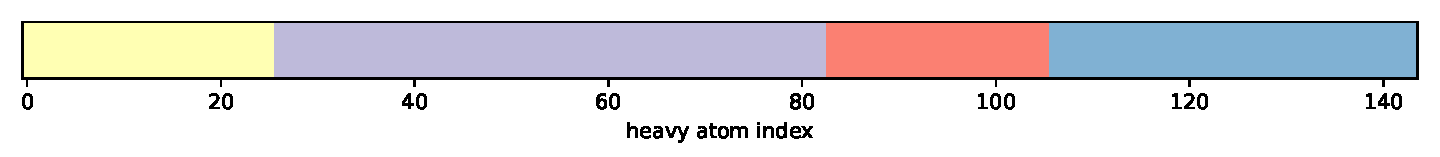
\includegraphics[width=0.7\textwidth]{2JOF_clustering_result_state_1.pdf}}\\
  \subfloat[Metastable State 2]{
  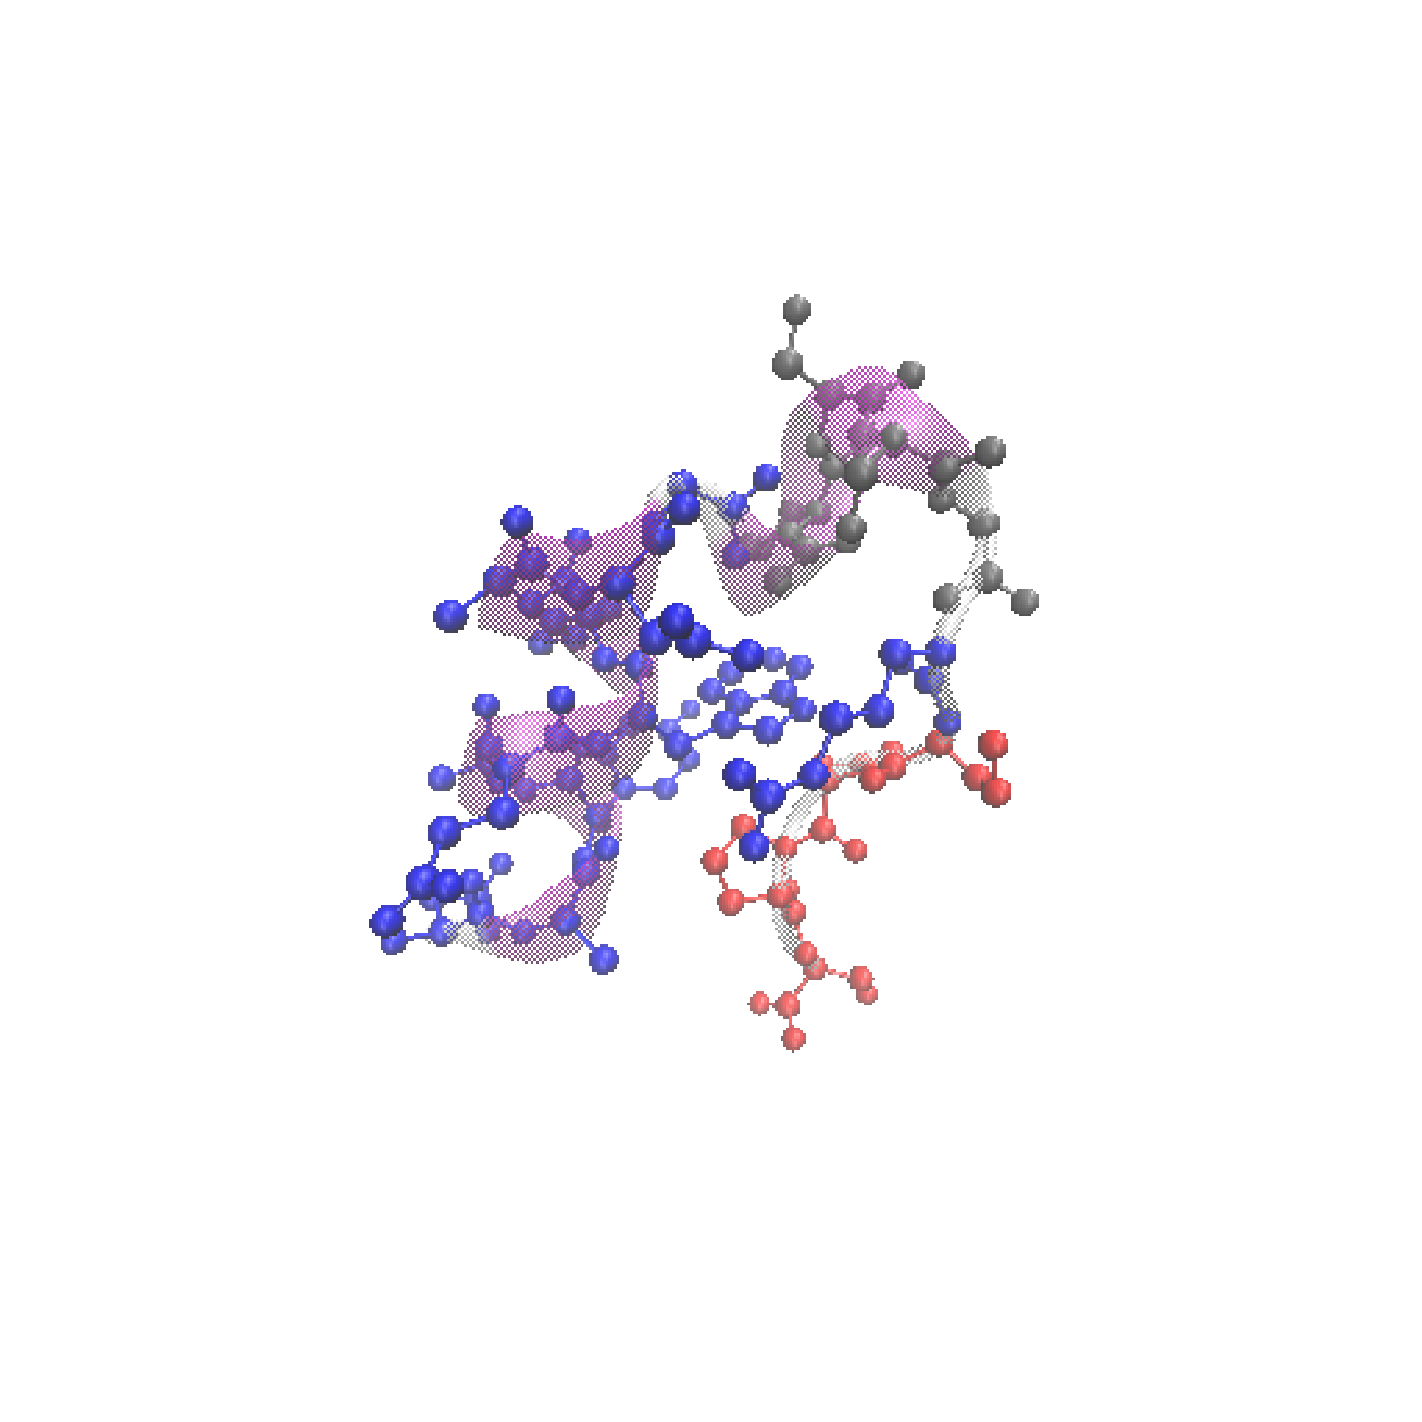
\includegraphics[width=0.3\textwidth, trim={5cm 5cm 5cm 5cm},clip]{2JOF_state_1.png}
  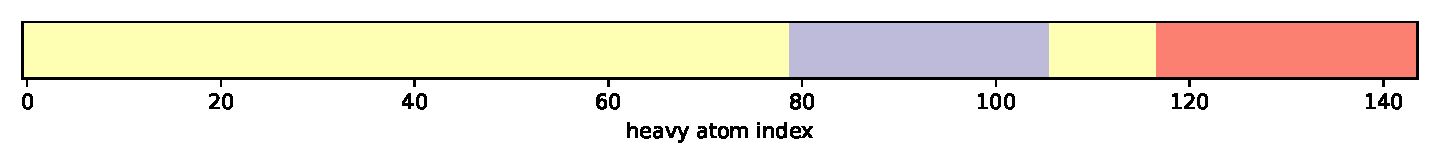
\includegraphics[width=0.7\textwidth]{2JOF_clustering_result_state_2.pdf}}\\
  \subfloat[Metastable State 3]{
  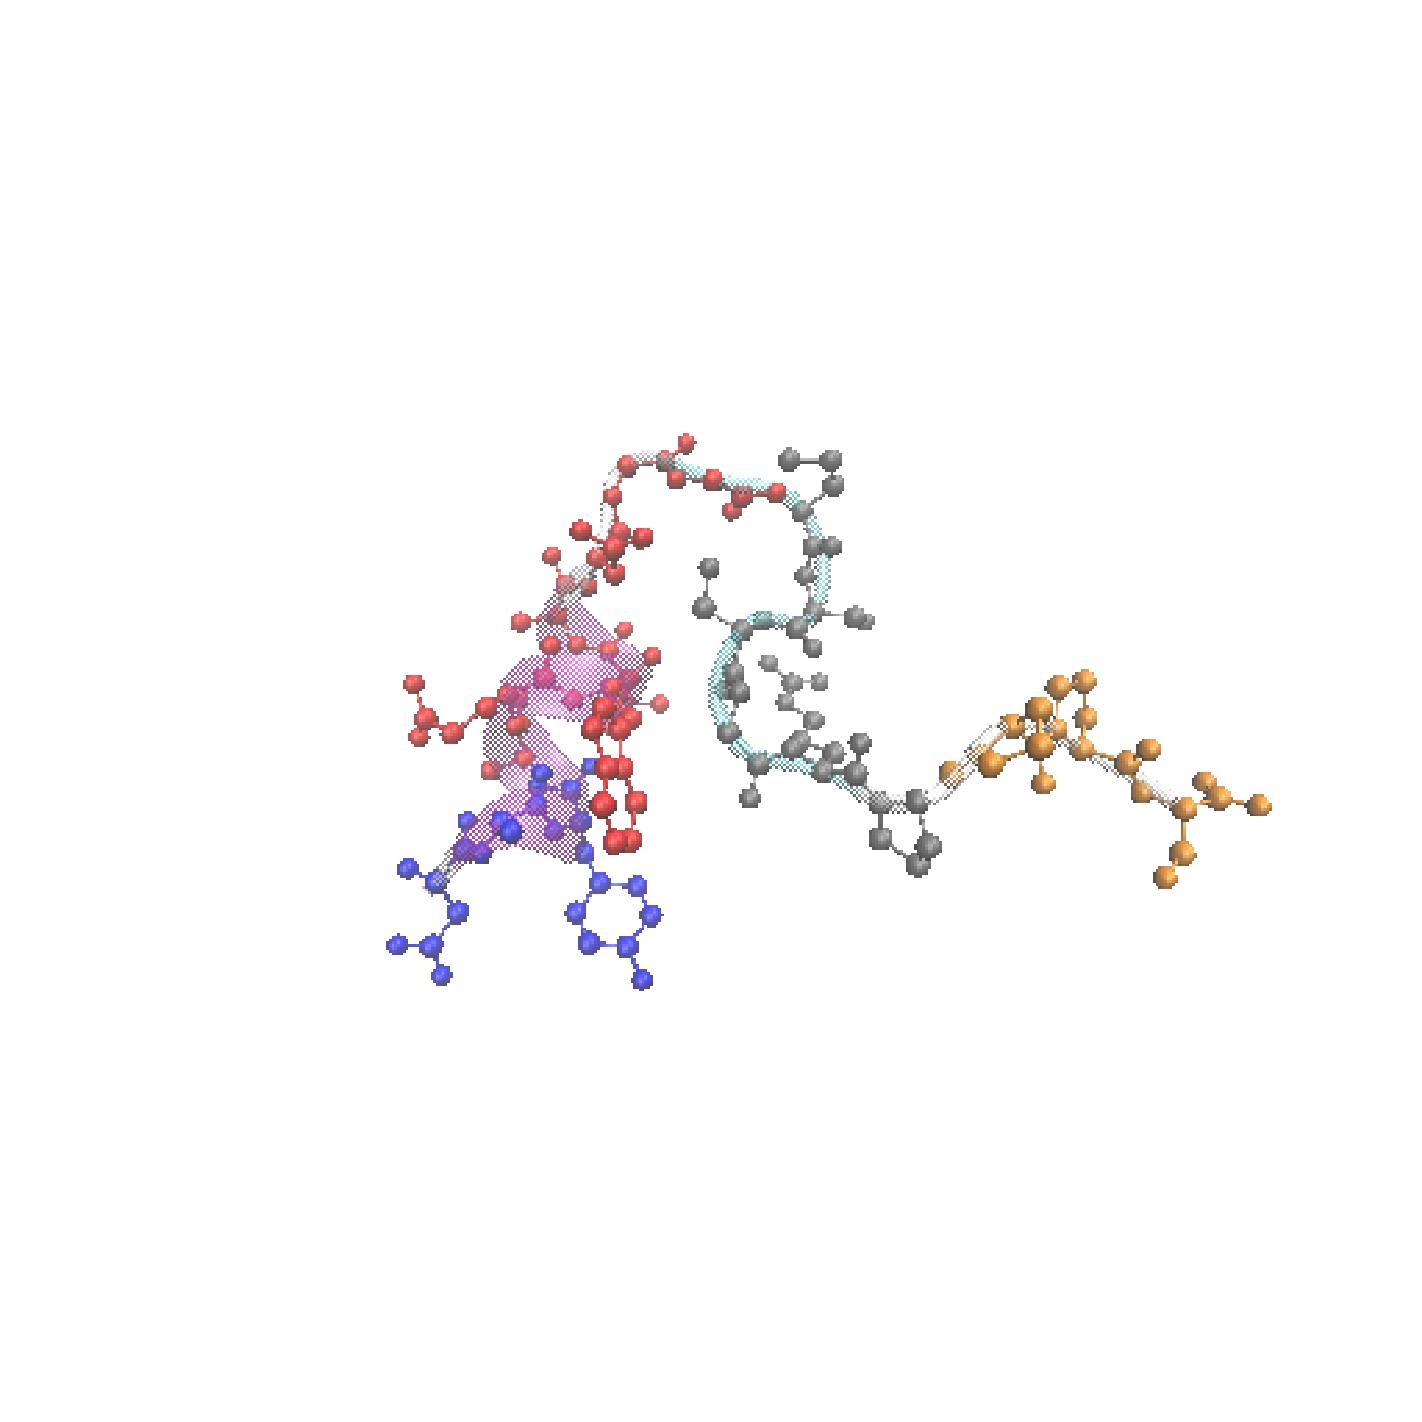
\includegraphics[width=0.3\textwidth, trim={5cm 5cm 5cm 5cm},clip]{2JOF_state_2.png}
  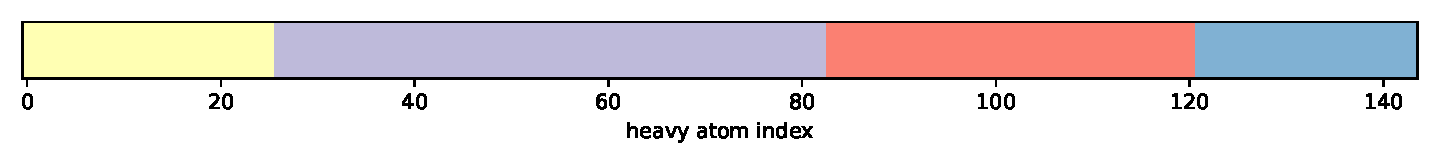
\includegraphics[width=0.7\textwidth]{2JOF_clustering_result_state_3.pdf}}\\
  \caption{\label{2JOF}Coherent domains for each metastable state of Trp-cage. Three metastable states are identified. For state 1 and 3, four coherent domains are obtained; for state 2, there are three.}
\end{figure}

\clearpage

\subsection*{BBA}

\begin{figure}[htbp]
  \centering
  \subfloat[Metastable State 1]{
  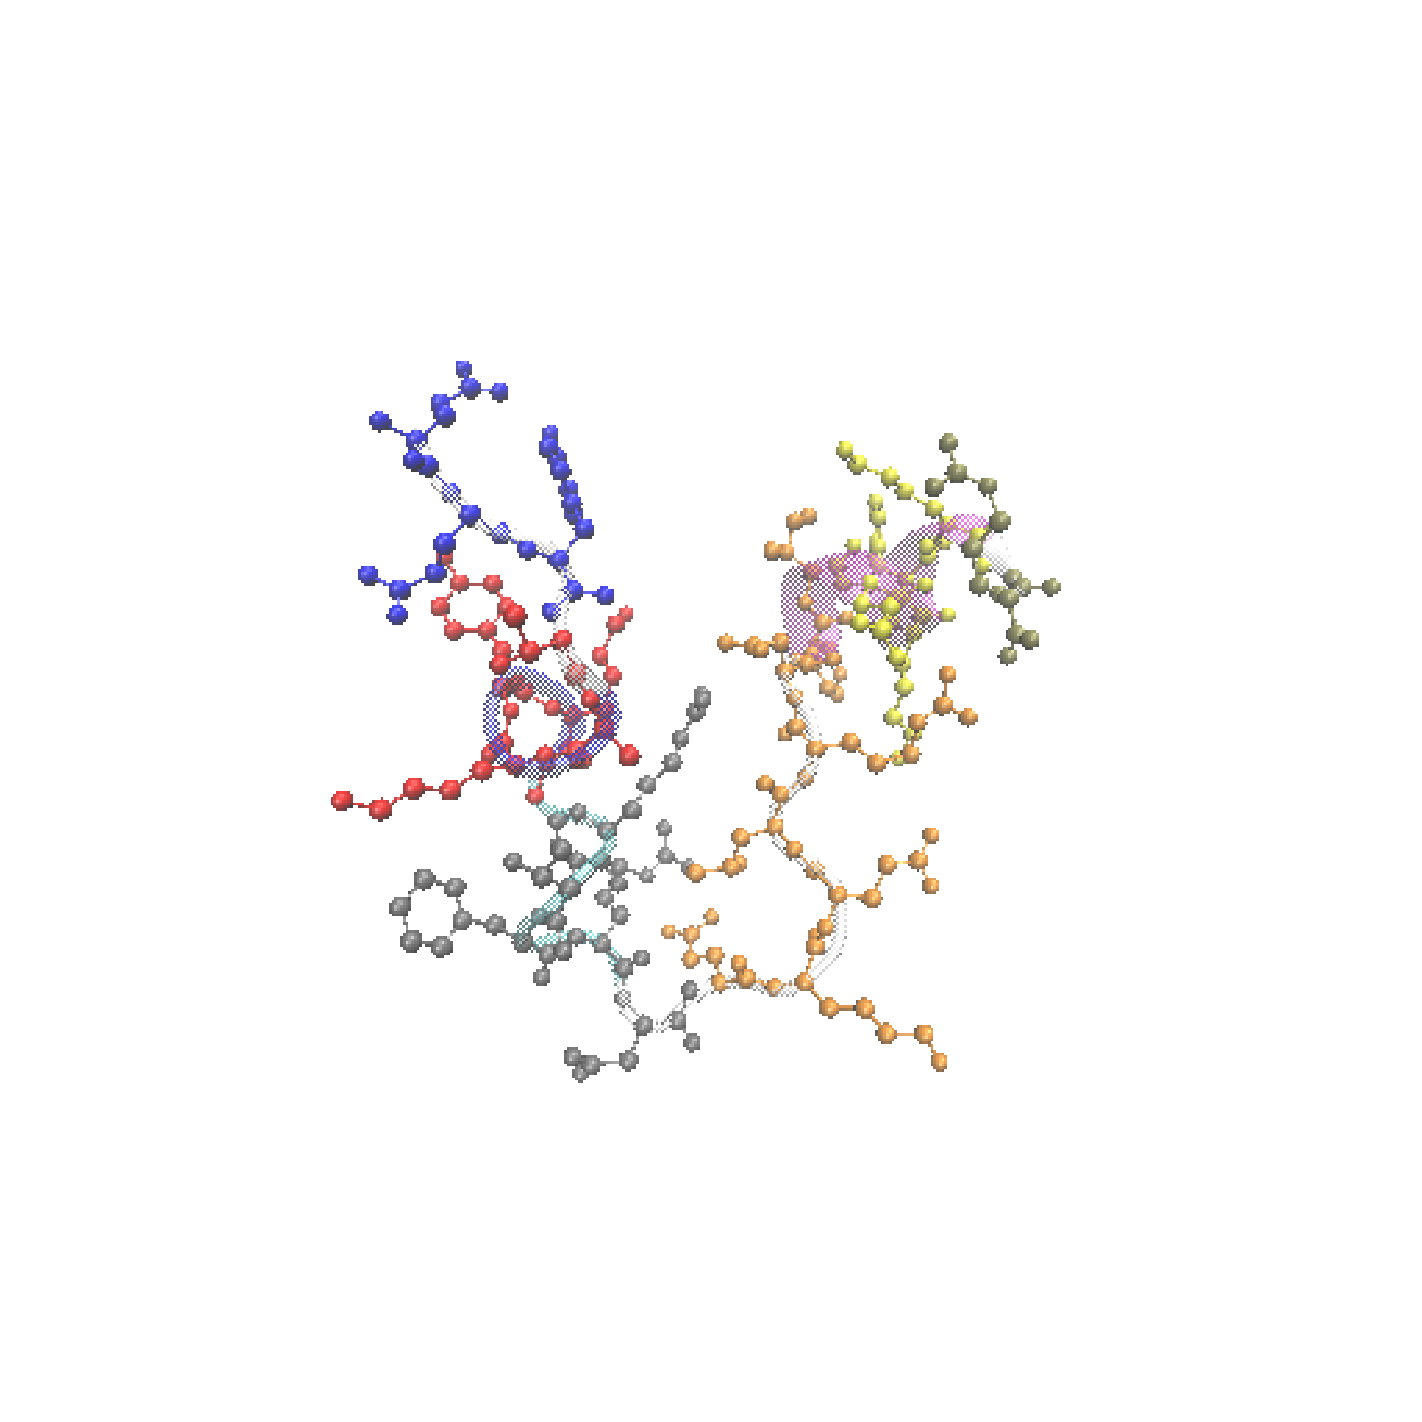
\includegraphics[width=0.3\textwidth, trim={5cm 5cm 5cm 5cm},clip]{1FME_state_0.png}
  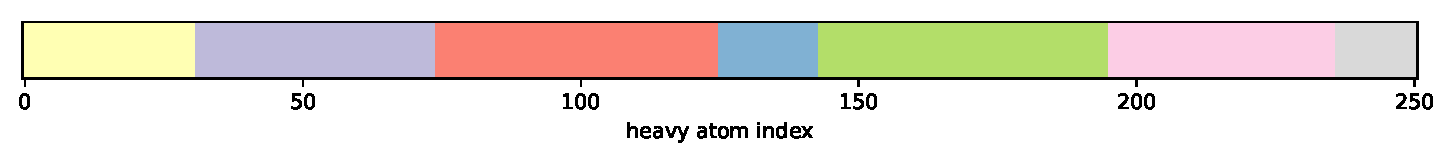
\includegraphics[width=0.7\textwidth]{1FME_clustering_result_state_1.pdf}}\\
  \subfloat[Metastable State 2]{
  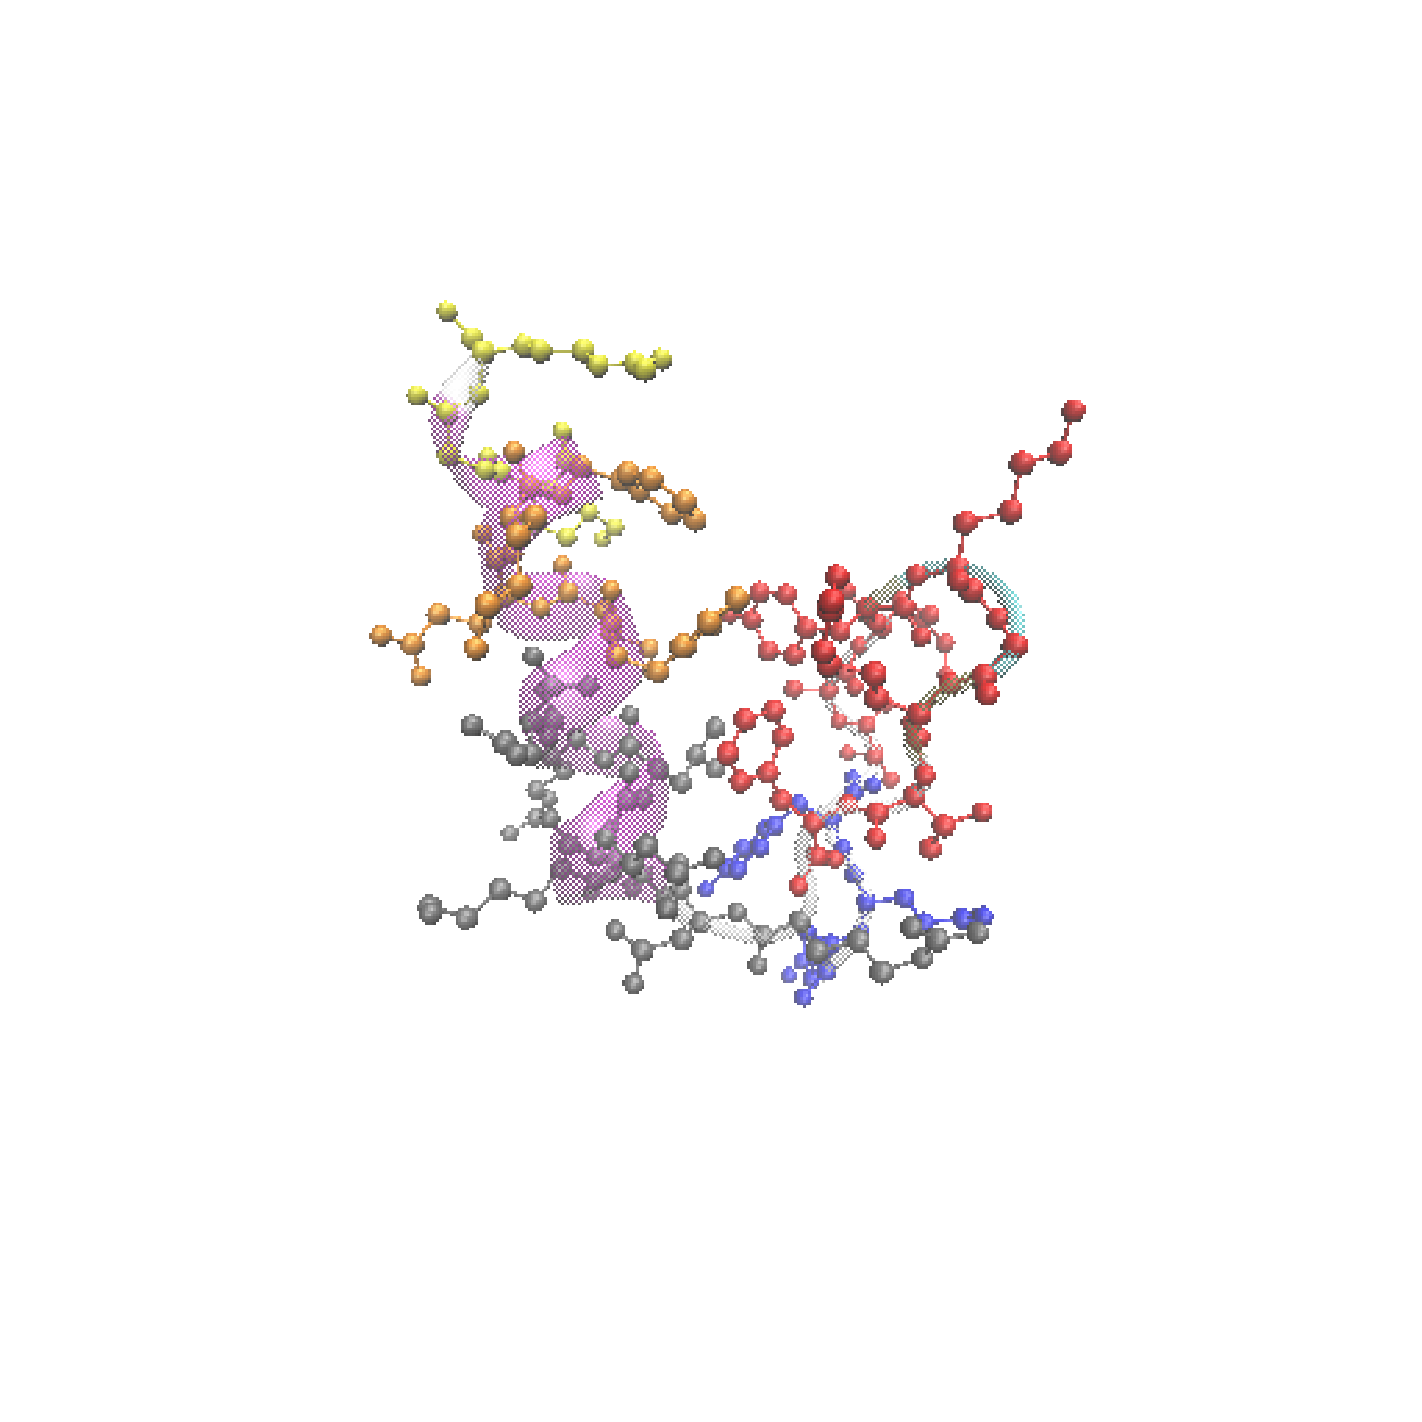
\includegraphics[width=0.3\textwidth, trim={5cm 5cm 5cm 5cm},clip]{1FME_state_1.png}
  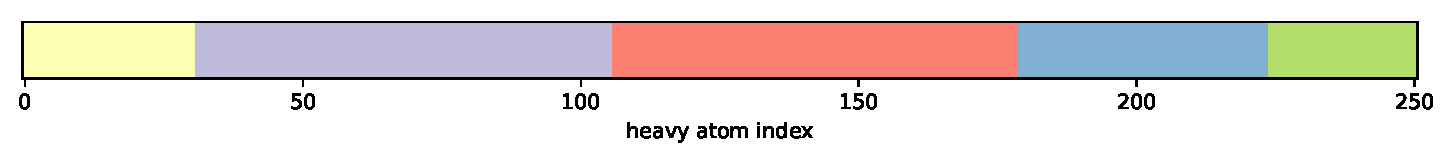
\includegraphics[width=0.7\textwidth]{1FME_clustering_result_state_2.pdf}}\\
  \caption{\label{1FME}Coherent domains for each metastable state of BBA. Two metastable states are identified. For state 1, seven coherent domains are obtained; for state 2 there are five.}
\end{figure}

\clearpage

\subsection*{Villin}

\begin{figure}[htbp]
  \centering
  \subfloat[Metastable State 1]{
  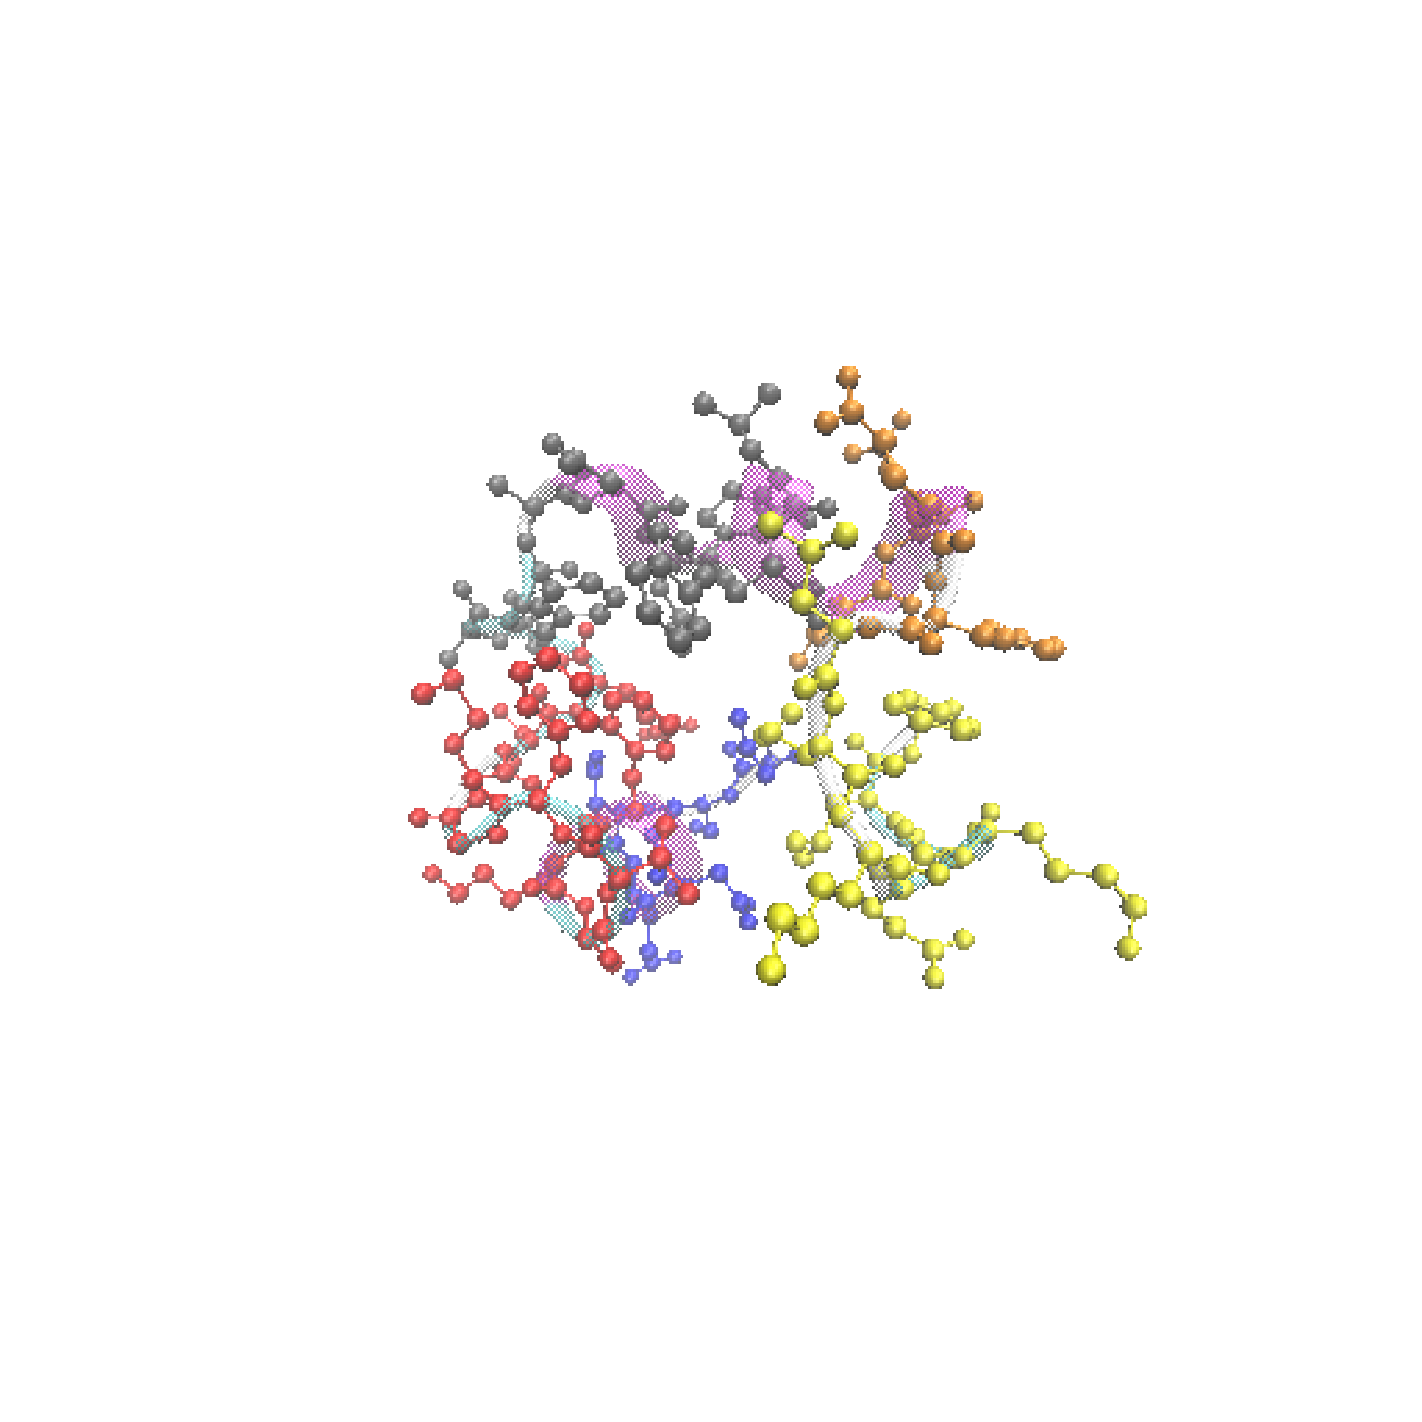
\includegraphics[width=0.3\textwidth, trim={5cm 5cm 5cm 5cm},clip]{2F4K_state_0.png}
  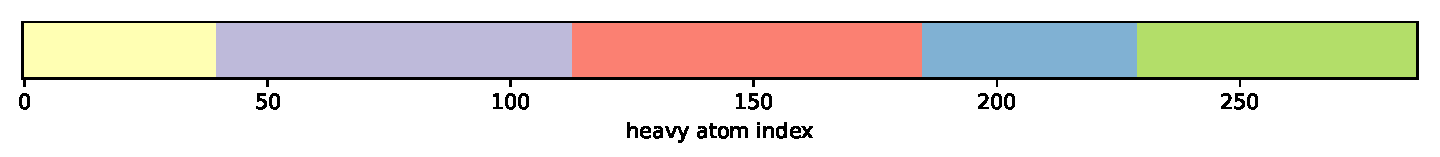
\includegraphics[width=0.7\textwidth]{2F4K_clustering_result_state_1.pdf}}\\
  \subfloat[Metastable State 2]{
  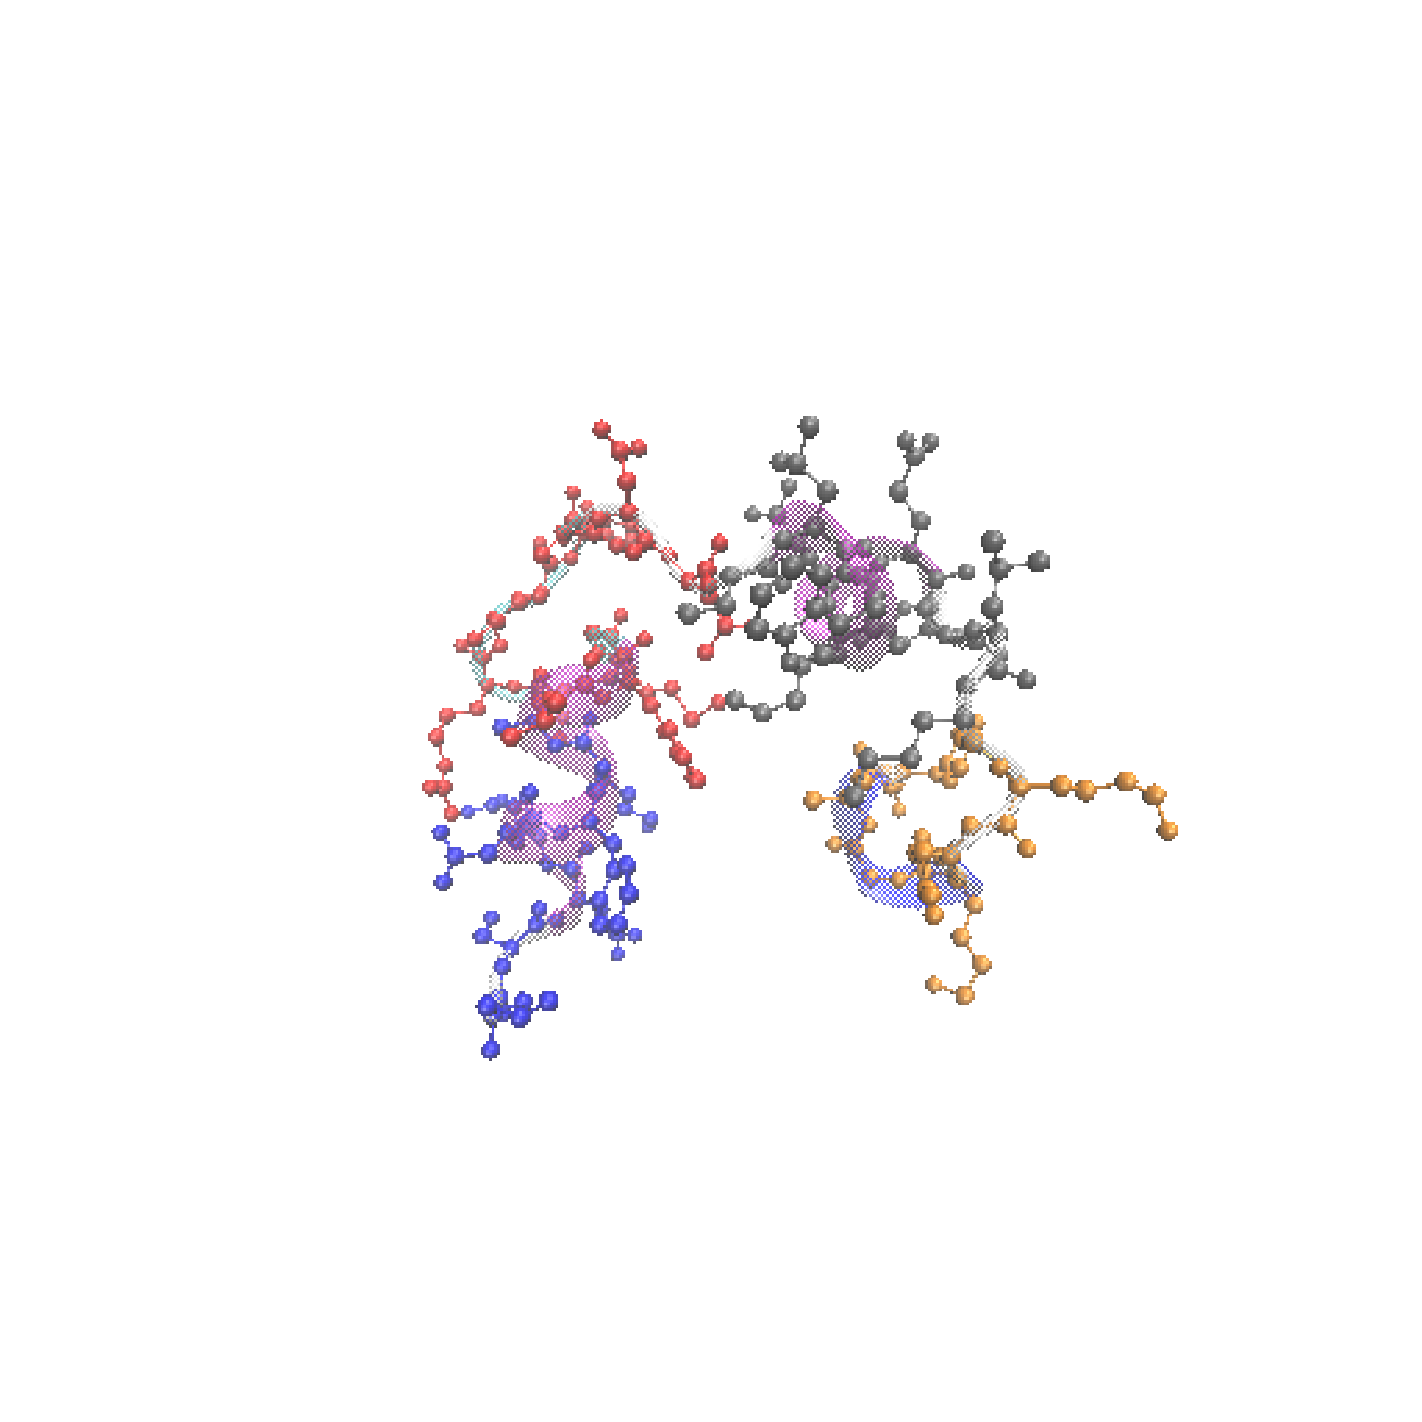
\includegraphics[width=0.3\textwidth, trim={5cm 5cm 5cm 5cm},clip]{2F4K_state_1.png}
  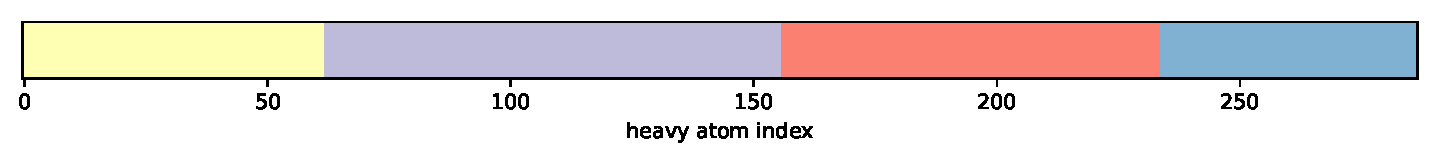
\includegraphics[width=0.7\textwidth]{2F4K_clustering_result_state_2.pdf}}\\
  \subfloat[Metastable State 3]{
  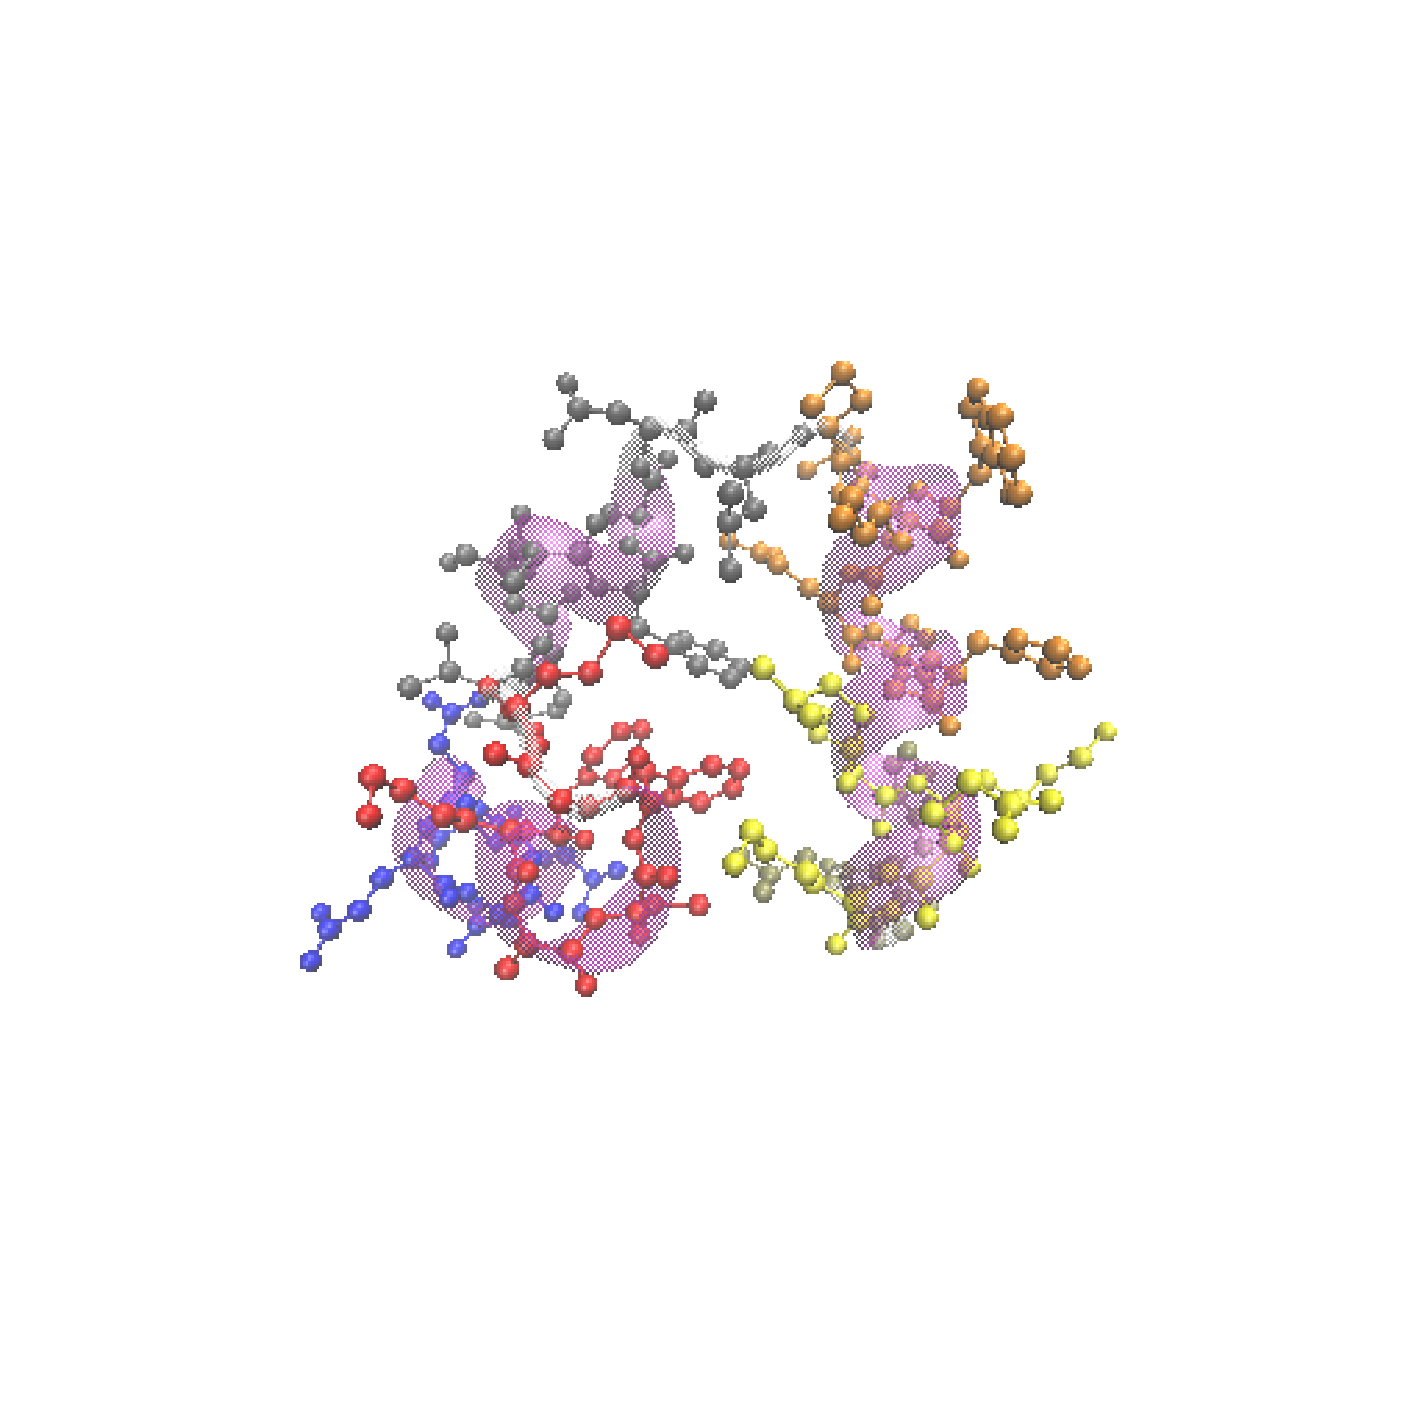
\includegraphics[width=0.3\textwidth, trim={5cm 5cm 5cm 5cm},clip]{2F4K_state_2.png}
  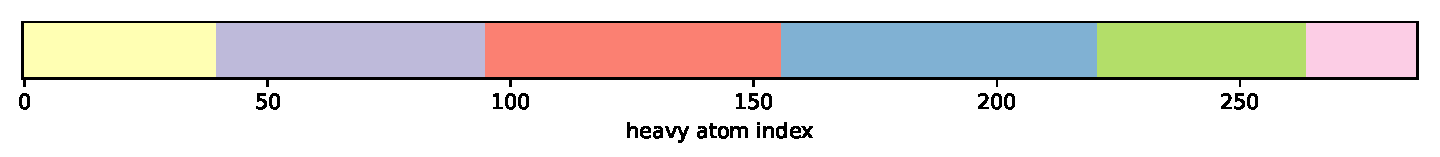
\includegraphics[width=0.7\textwidth]{2F4K_clustering_result_state_3.pdf}}\\
  \caption{\label{2F4K}Coherent domains for each metastable state of Villin. Three metastable states are identified. For state 1, 2 and 3, five, four and six coherent domains are obtained respectively.}
\end{figure}

\clearpage

\subsection*{BBL}

\begin{figure}[htbp]
  \centering
  \subfloat[Metastable State 1]{
  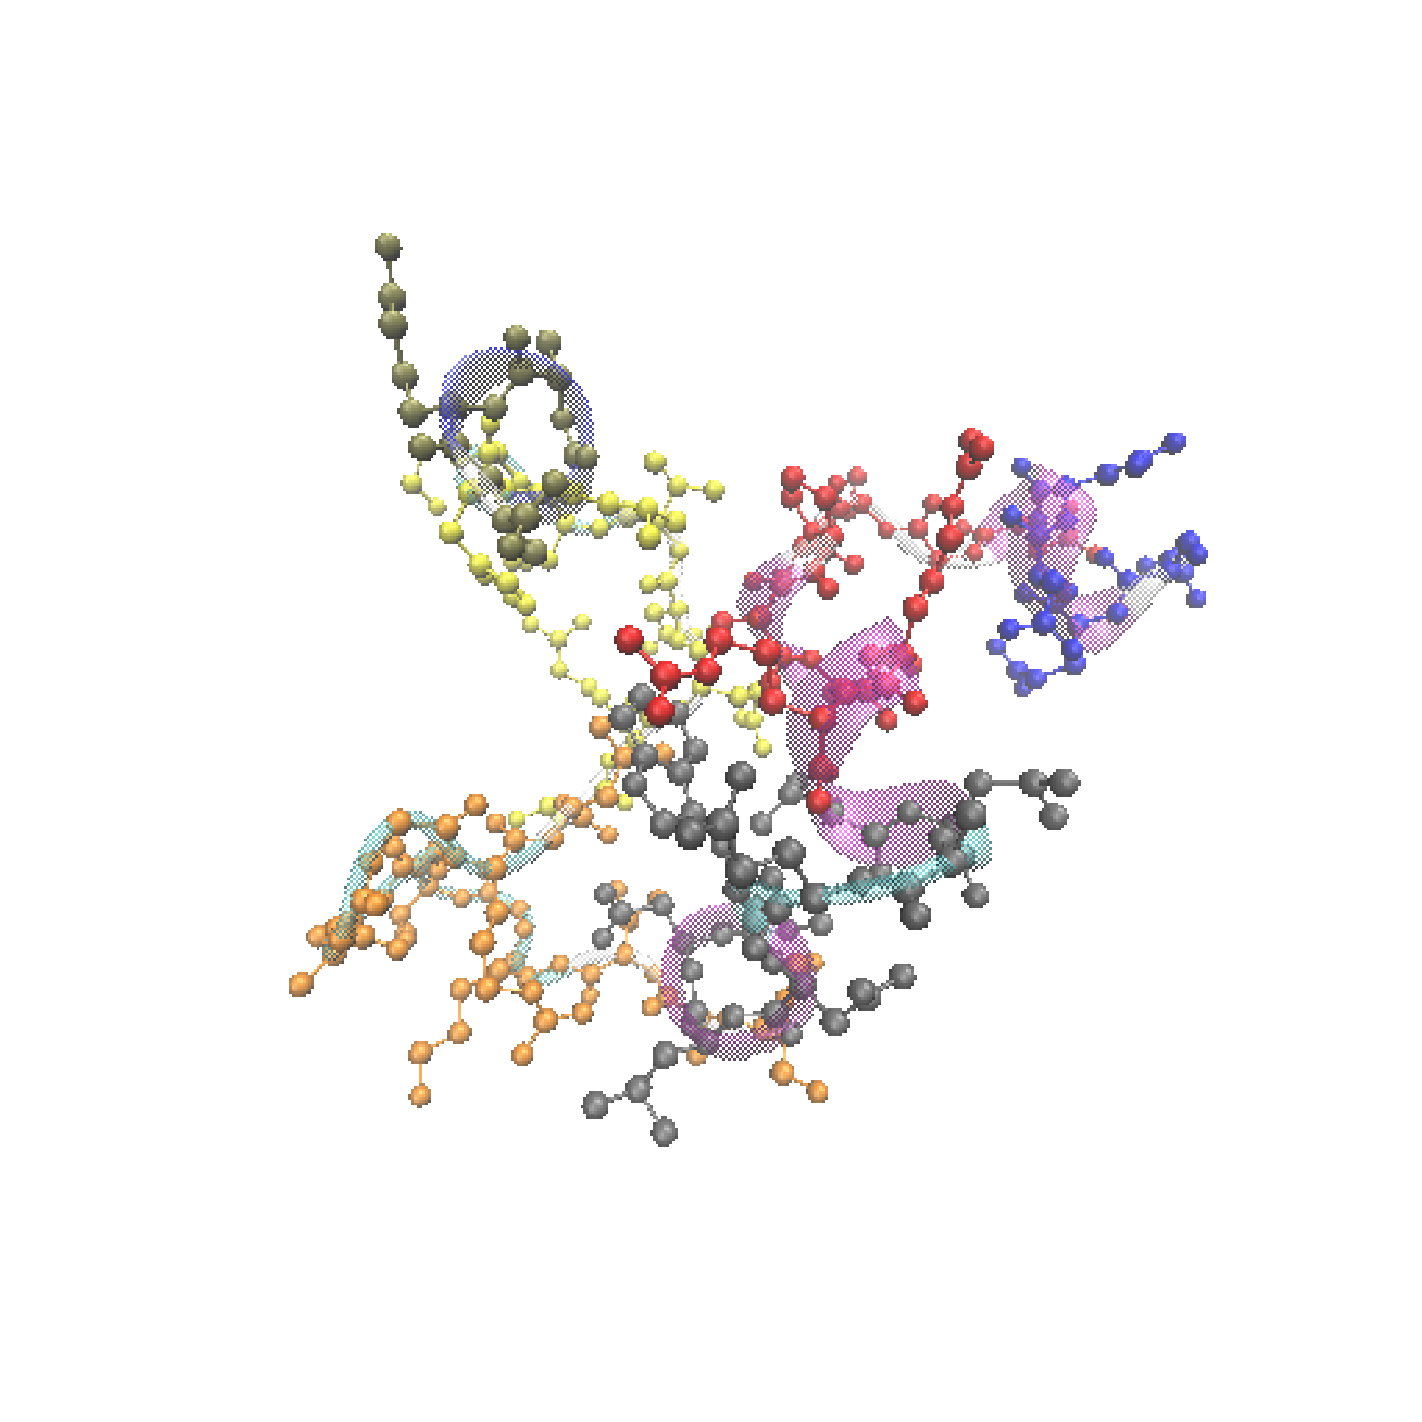
\includegraphics[width=0.3\textwidth, trim={5cm 5cm 5cm 5cm},clip]{2WAV_state_0.png}
  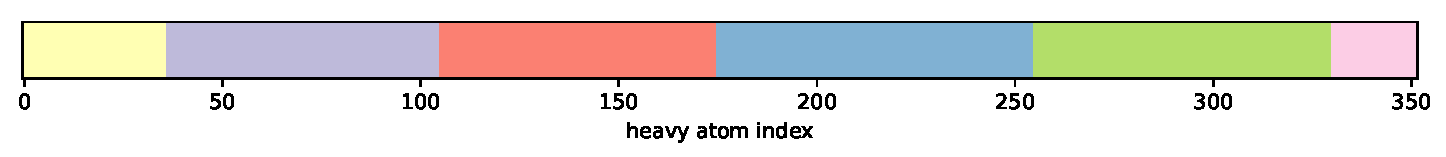
\includegraphics[width=0.7\textwidth]{2WAV_clustering_result_state_1.pdf}}\\
  \subfloat[Metastable State 2]{
  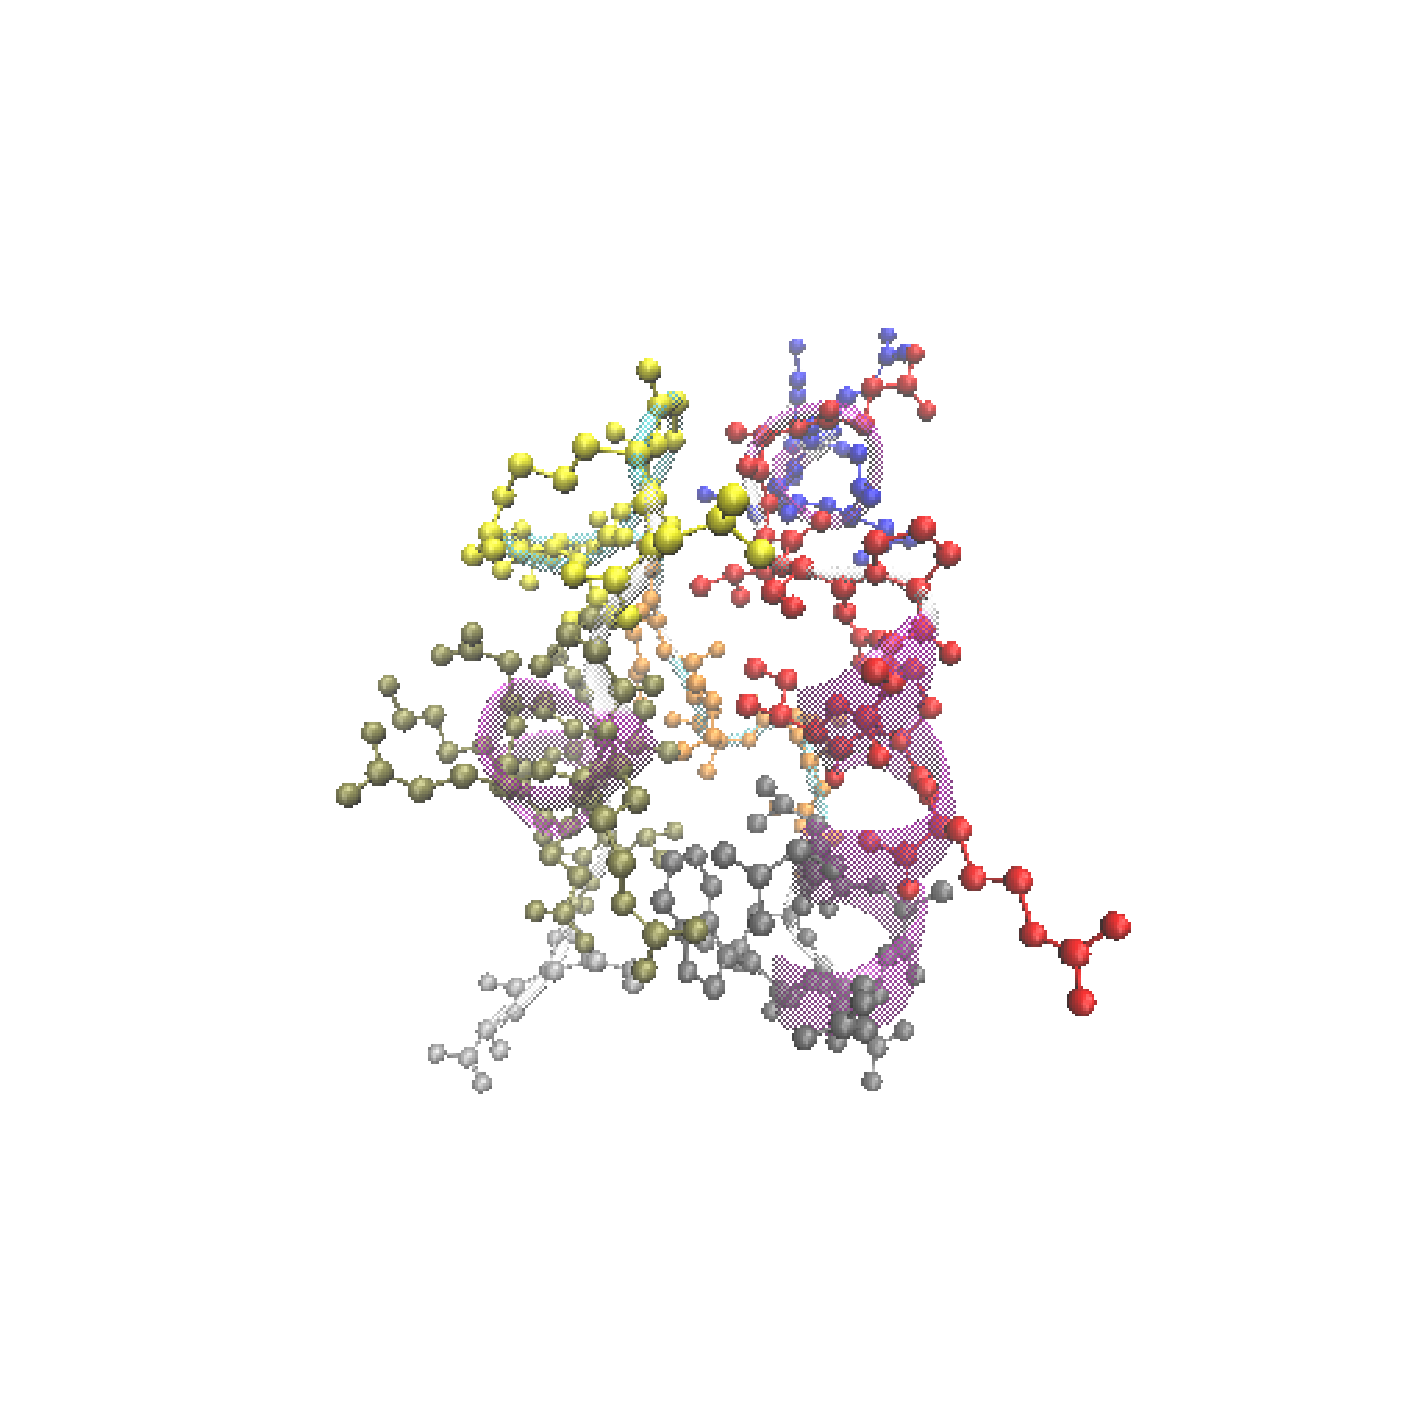
\includegraphics[width=0.3\textwidth, trim={5cm 5cm 5cm 5cm},clip]{2WAV_state_1.png}
  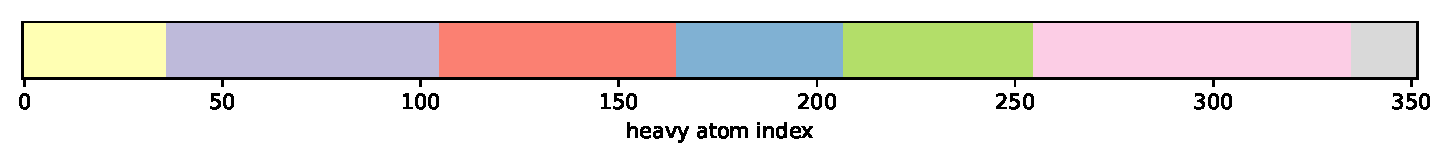
\includegraphics[width=0.7\textwidth]{2WAV_clustering_result_state_2.pdf}}\\
  \subfloat[Metastable State 3]{
  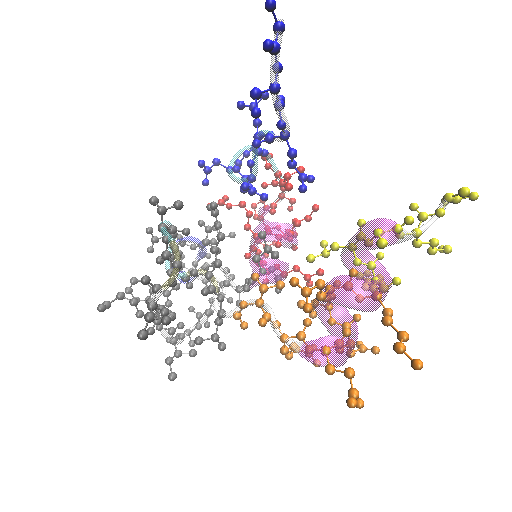
\includegraphics[width=0.3\textwidth, trim={0cm 0cm 0cm 0cm},clip]{2WAV_state_2.png}
  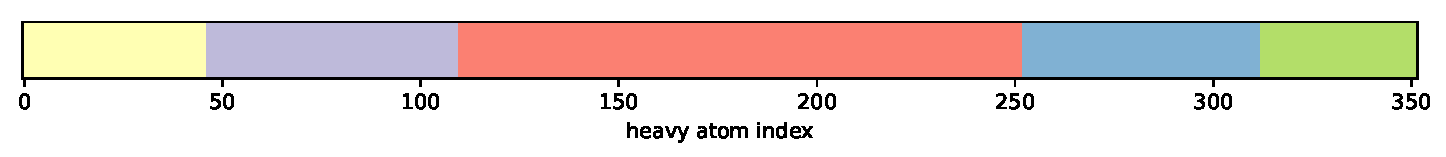
\includegraphics[width=0.7\textwidth]{2WAV_clustering_result_state_3.pdf}}\\
\end{figure}

%\addtocounter{figure}{-1}

\begin{figure}[htbp]
  \addtocounter{subfigure}{3}
  \subfloat[Metastable State 4]{
  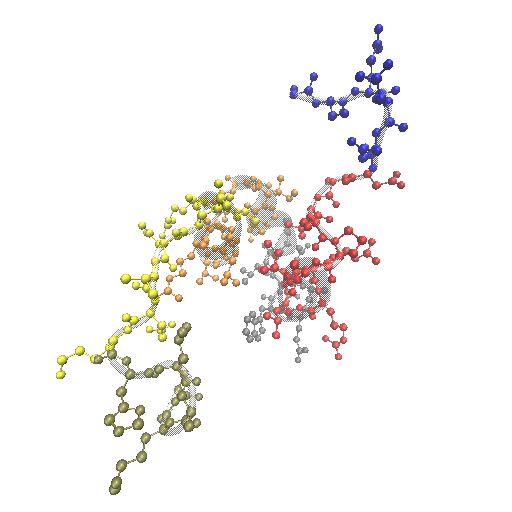
\includegraphics[width=0.3\textwidth, trim={0cm 0cm 0cm 0cm},clip]{2WAV_state_3.png}
  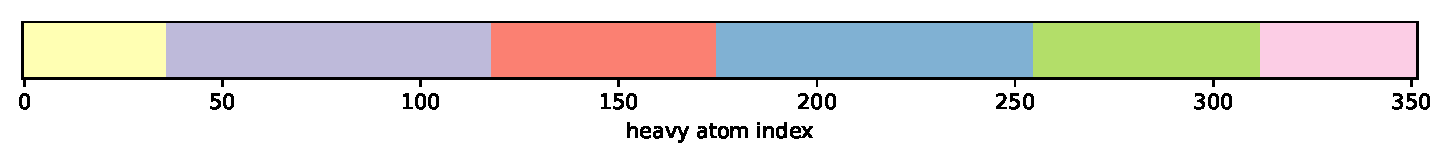
\includegraphics[width=0.7\textwidth]{2WAV_clustering_result_state_4.pdf}}\\
  \caption{\label{2WAV}Coherent domains for each metastable state of BBL. Four metastable states are identified. For state 1 and 4, six coherent domains are obtained; for state 2 and 3, there seven and five respectively.}
\end{figure}

\clearpage

\subsection*{Protein B}

\begin{figure}[htbp]
  \centering
  \subfloat[Metastable State 1]{
  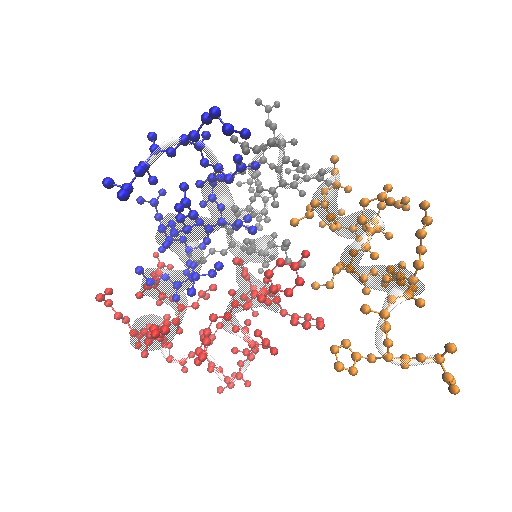
\includegraphics[width=0.3\textwidth, trim={0cm 0cm 0cm 0cm},clip]{PRB_state_0.png}
  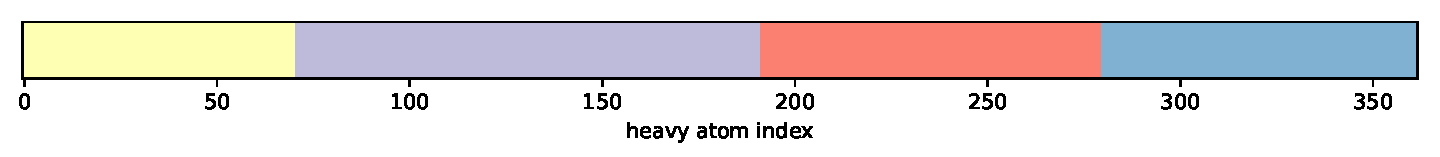
\includegraphics[width=0.7\textwidth]{PRB_clustering_result_state_1.pdf}}\\
  \subfloat[Metastable State 2]{
  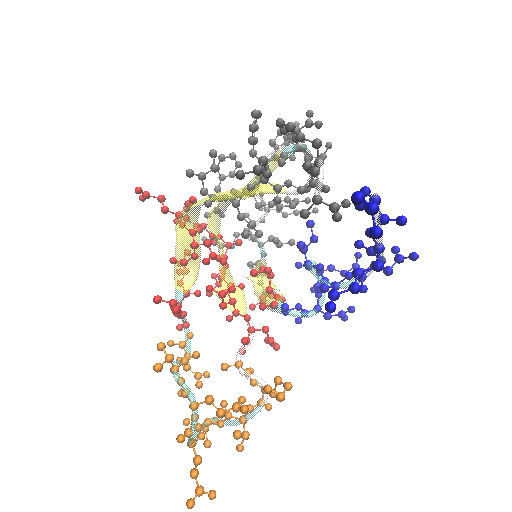
\includegraphics[width=0.3\textwidth, trim={0cm 0cm 0cm 0cm},clip]{PRB_state_1.png}
  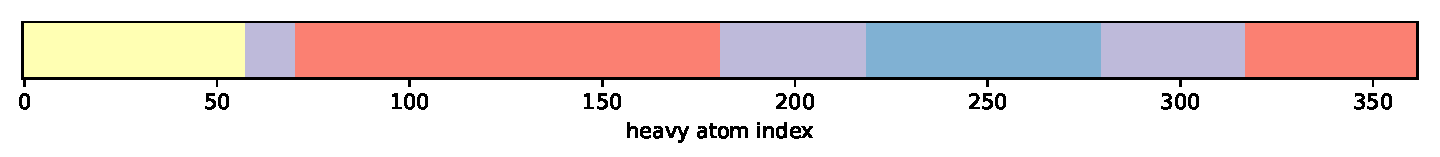
\includegraphics[width=0.7\textwidth]{PRB_clustering_result_state_2.pdf}}\\
  \subfloat[Metastable State 3]{
  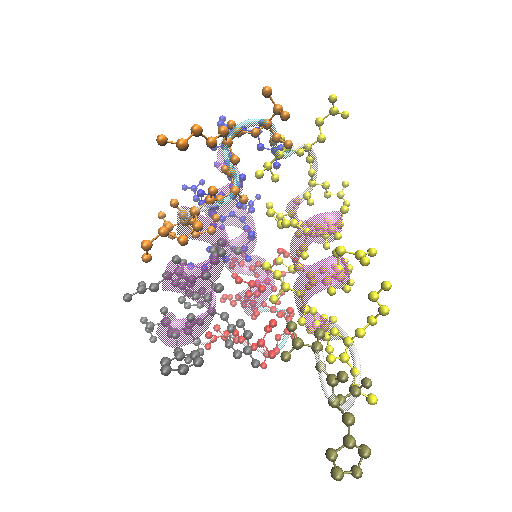
\includegraphics[width=0.3\textwidth, trim={0cm 0cm 0cm 0cm},clip]{PRB_state_2.png}
  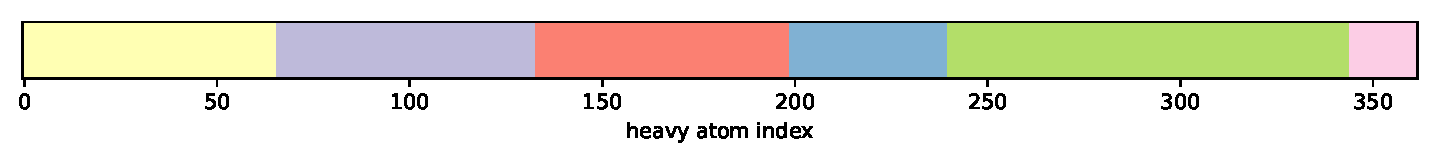
\includegraphics[width=0.7\textwidth]{PRB_clustering_result_state_3.pdf}}\\
  \caption{\label{PRB}Coherent domains for each metastable state of Protein B. Three metastable states are identified. For state 1 and 2, four coherent domains are obtained; for state 3, there are six.}
\end{figure}

\clearpage

\subsection*{Homeodomain}

\begin{figure}[htbp]
  \centering
  \subfloat[Metastable State 1]{
  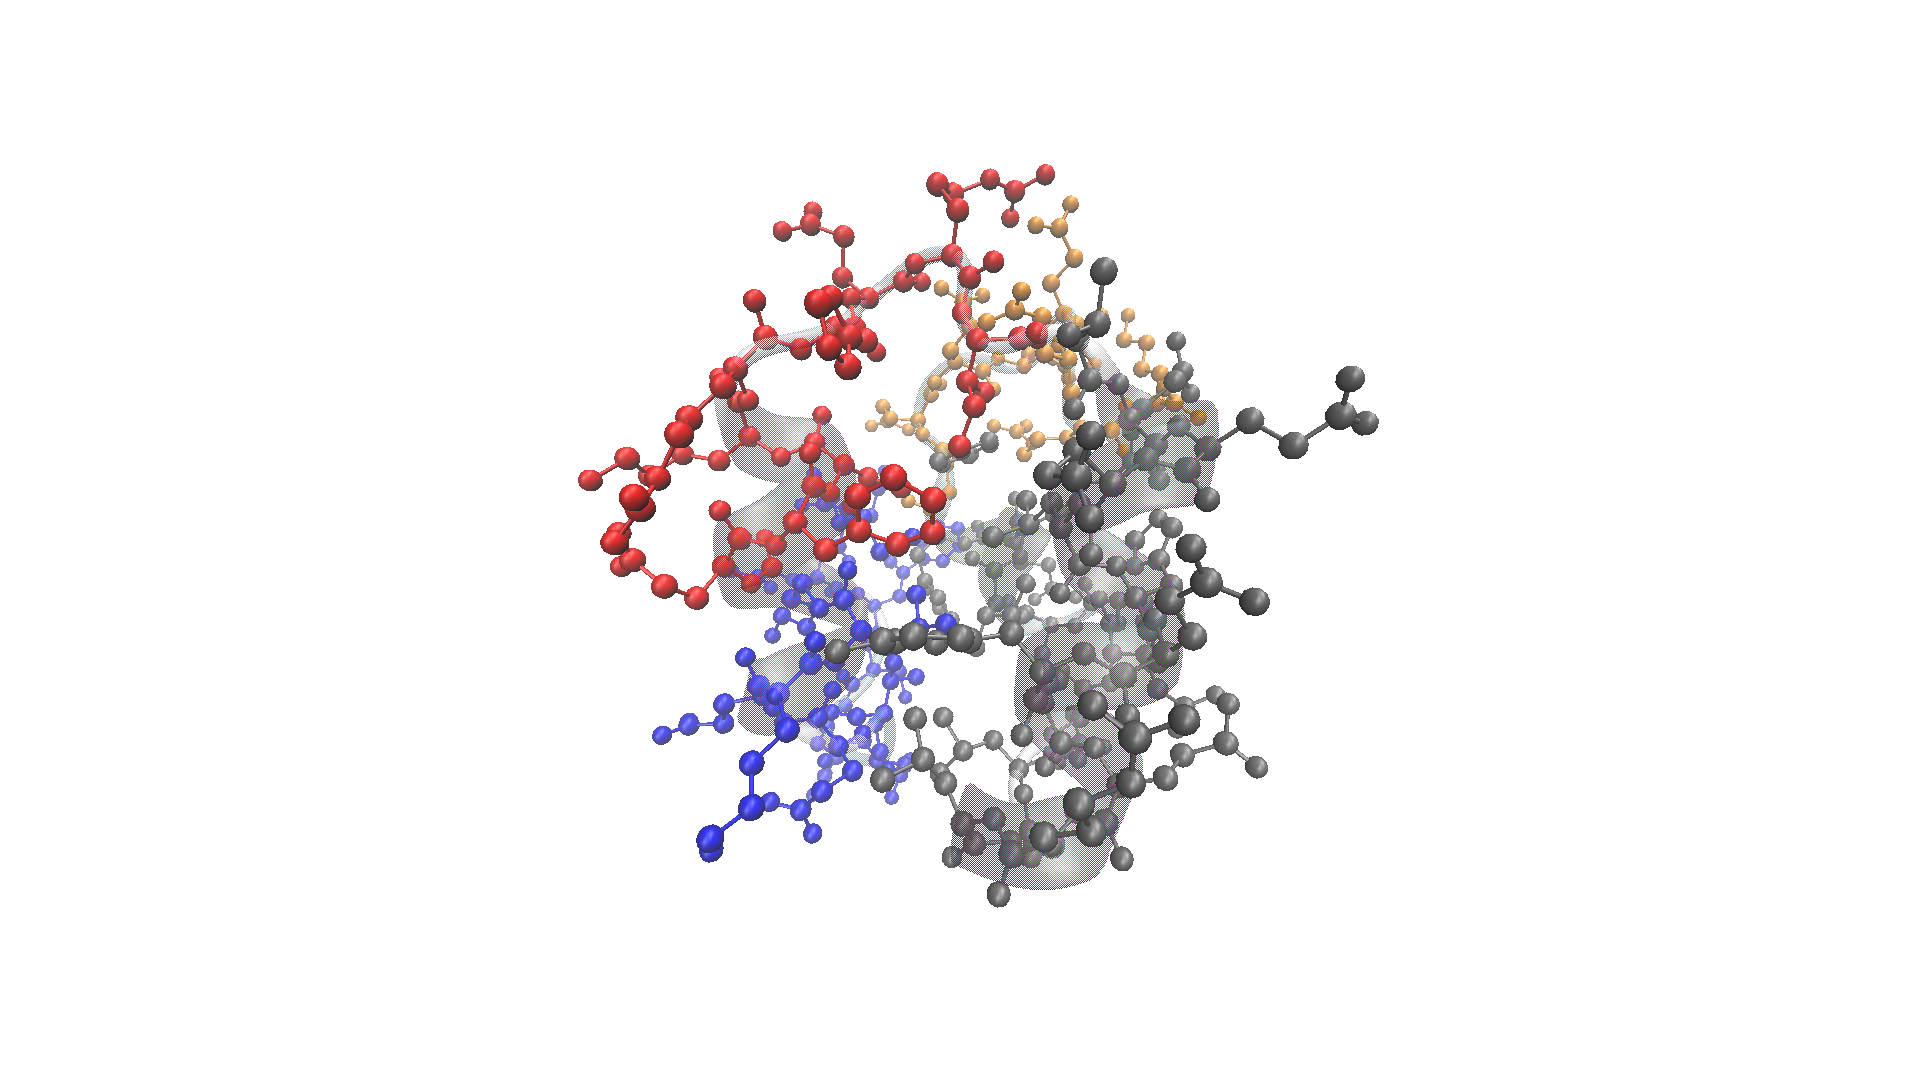
\includegraphics[width=0.3\textwidth, trim={14.815cm 0cm 14.815cm 0cm},clip]{UVF_state_0.png}
  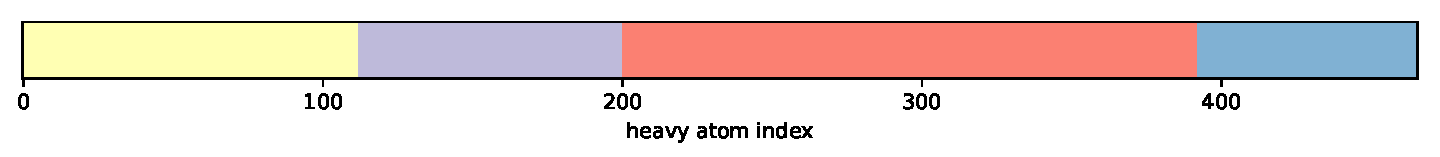
\includegraphics[width=0.7\textwidth]{UVF_clustering_result_state_1.pdf}}\\
  \subfloat[Metastable State 2]{
  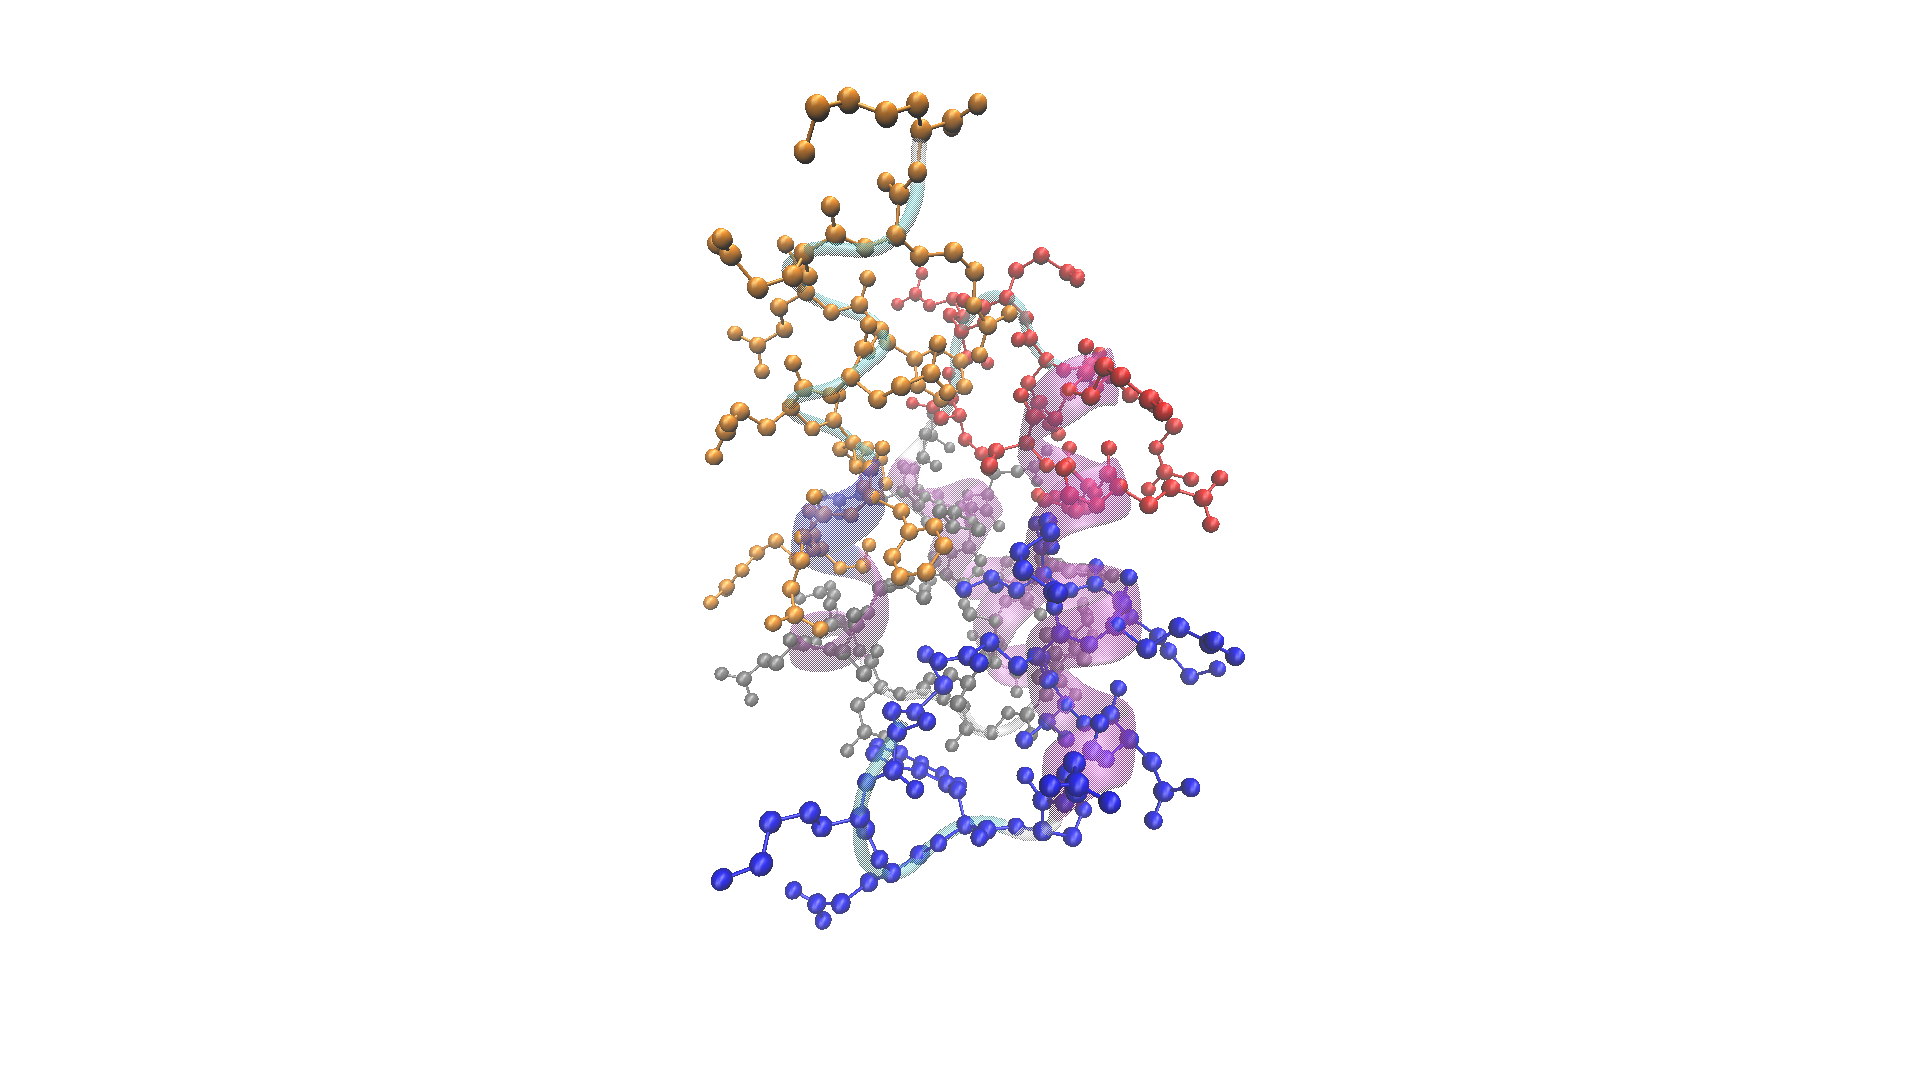
\includegraphics[width=0.3\textwidth, trim={14.815cm 0cm 14.815cm 0cm},clip]{UVF_state_1.png}
  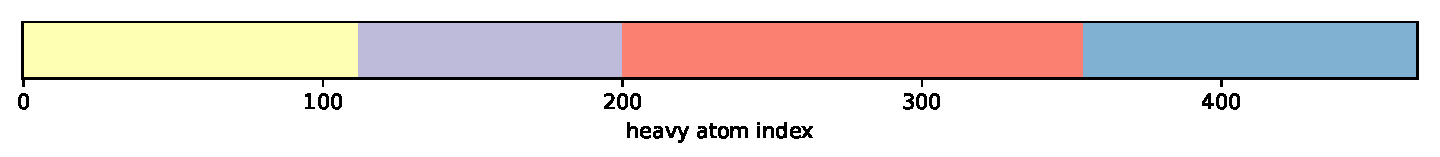
\includegraphics[width=0.7\textwidth]{UVF_clustering_result_state_2.pdf}}\\
  \subfloat[Metastable State 3]{
  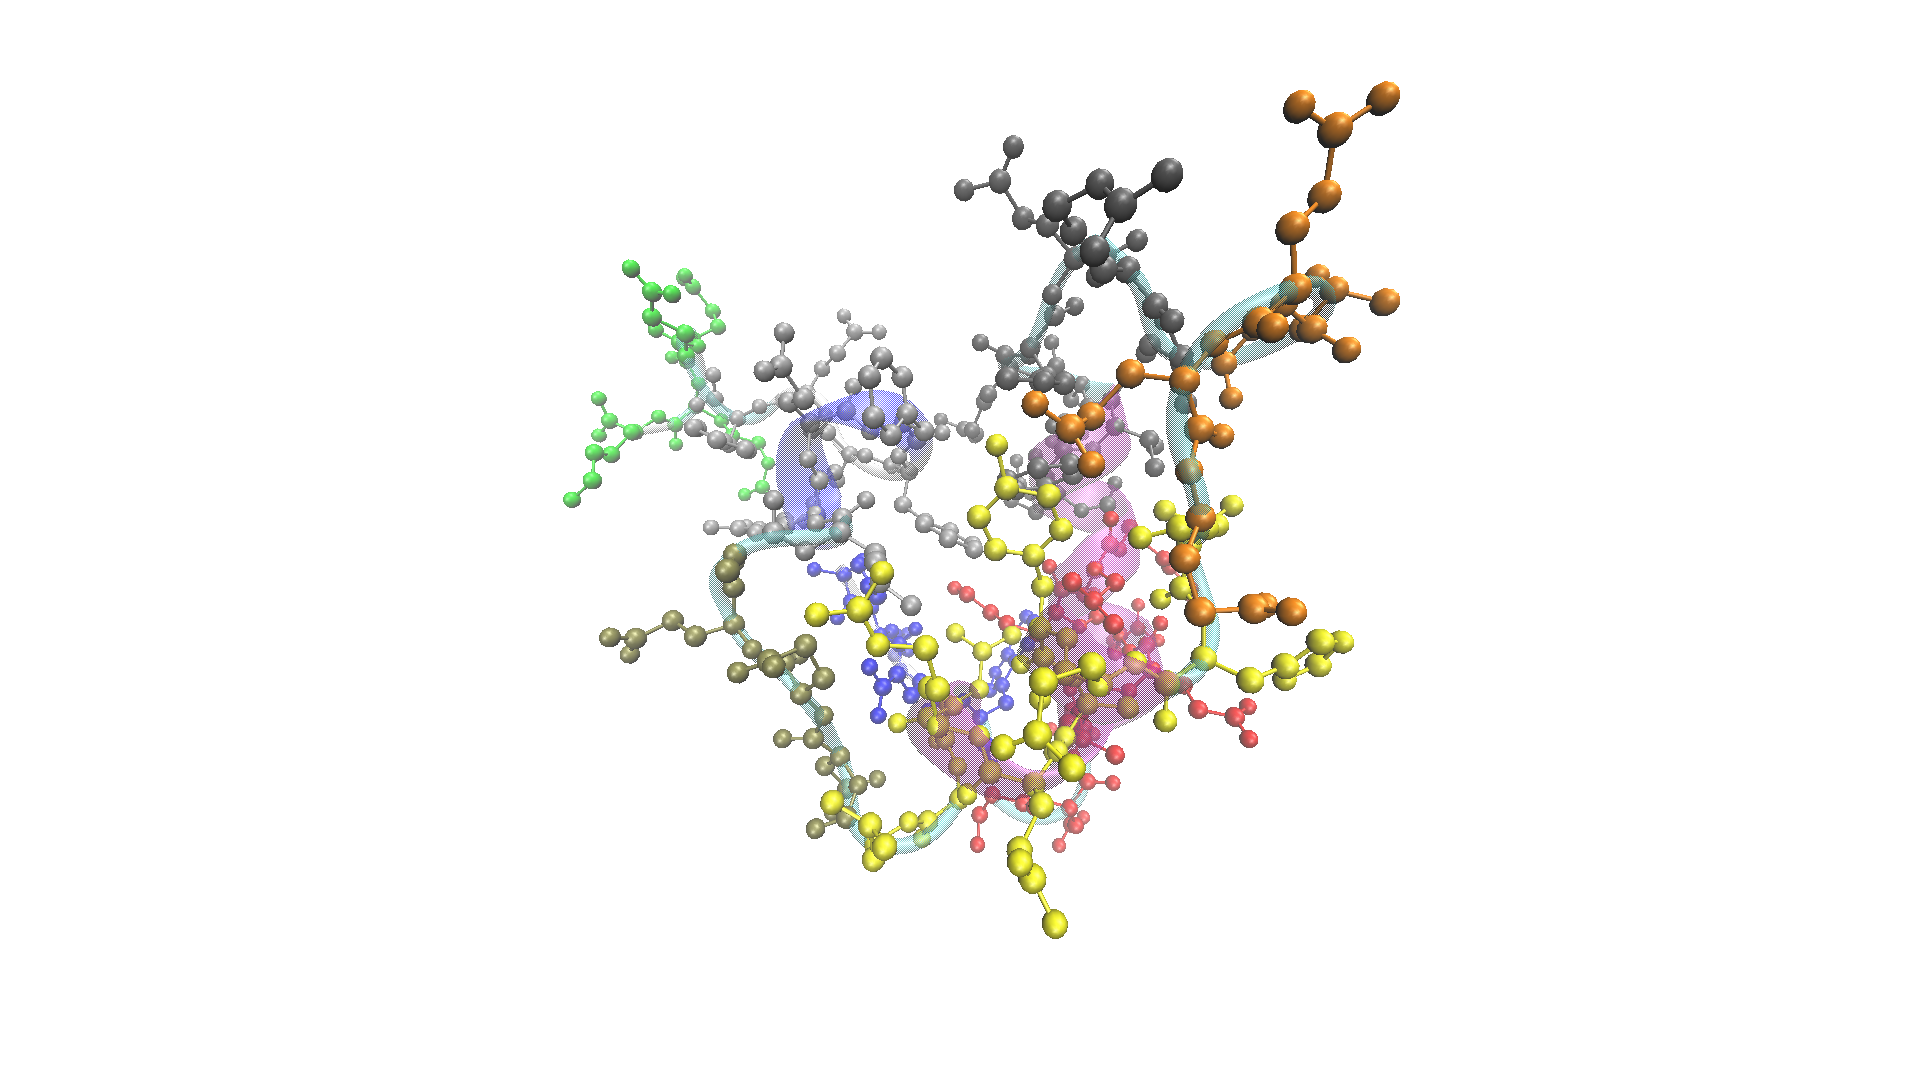
\includegraphics[width=0.3\textwidth, trim={14.815cm 0cm 14.815cm 0cm},clip]{UVF_state_2.png}
  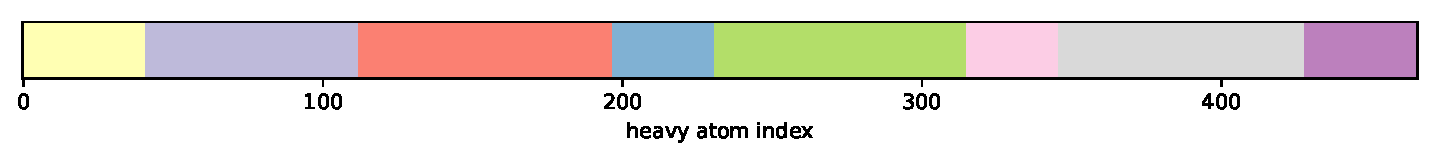
\includegraphics[width=0.7\textwidth]{UVF_clustering_result_state_3.pdf}}\\
  \caption{\label{UVF}Coherent domains for each metastable state of Homeodomain. Three metastable states are identified. For state 1 and 2, four coherent domains are obtained; for state 3, there are eight.}
\end{figure}

\clearpage

\subsection*{Protein G}

\begin{figure}[htbp]
  \centering
  \subfloat[Metastable State 1]{
  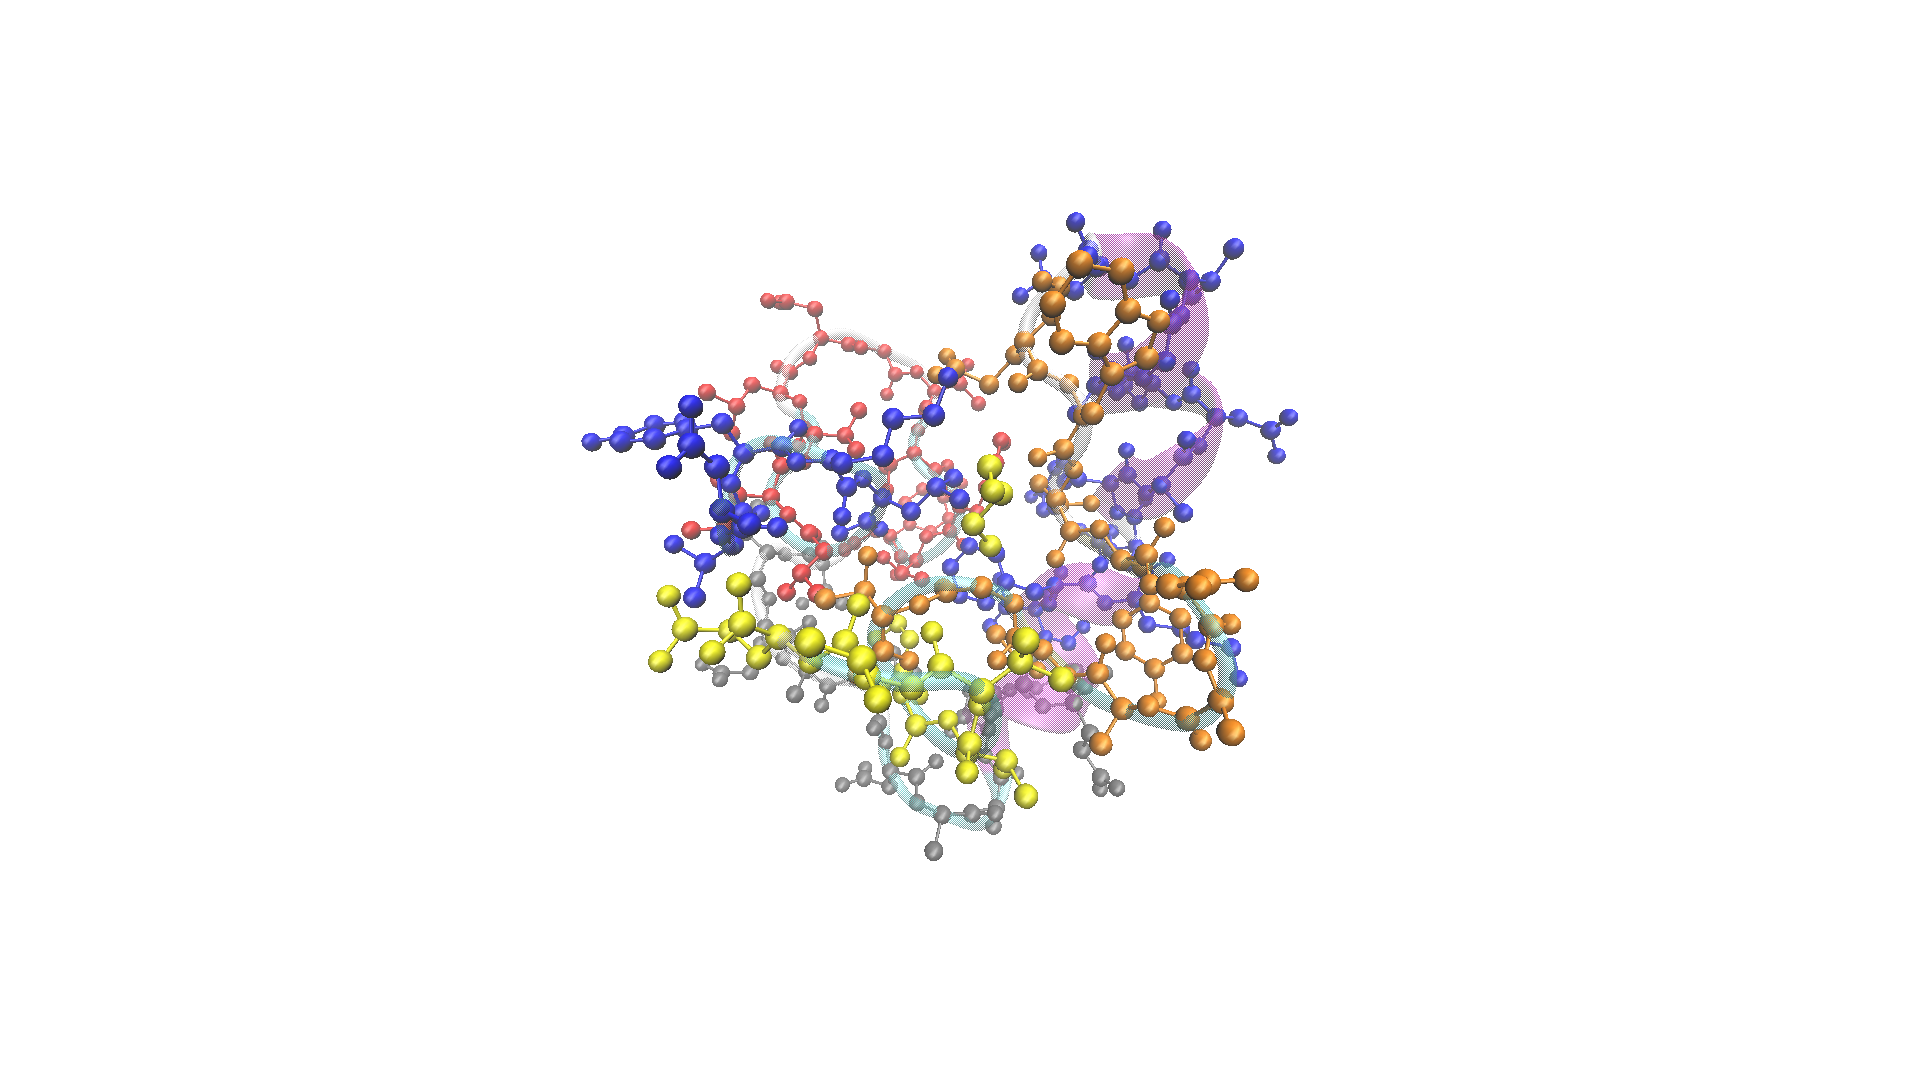
\includegraphics[width=0.3\textwidth, trim={14.815cm 0cm 14.815cm 0cm},clip]{NuG2_state_0.png}
  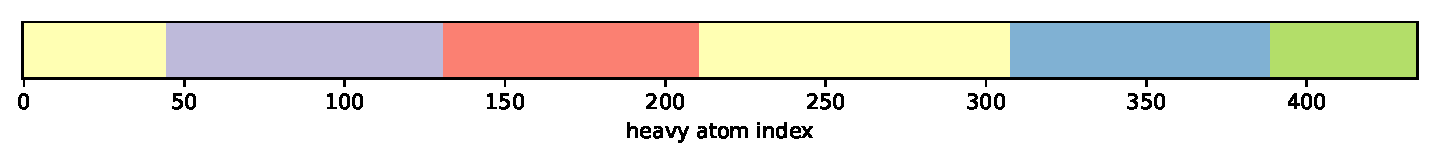
\includegraphics[width=0.7\textwidth]{NuG2_clustering_result_state_1.pdf}}\\
  \subfloat[Metastable State 2]{
  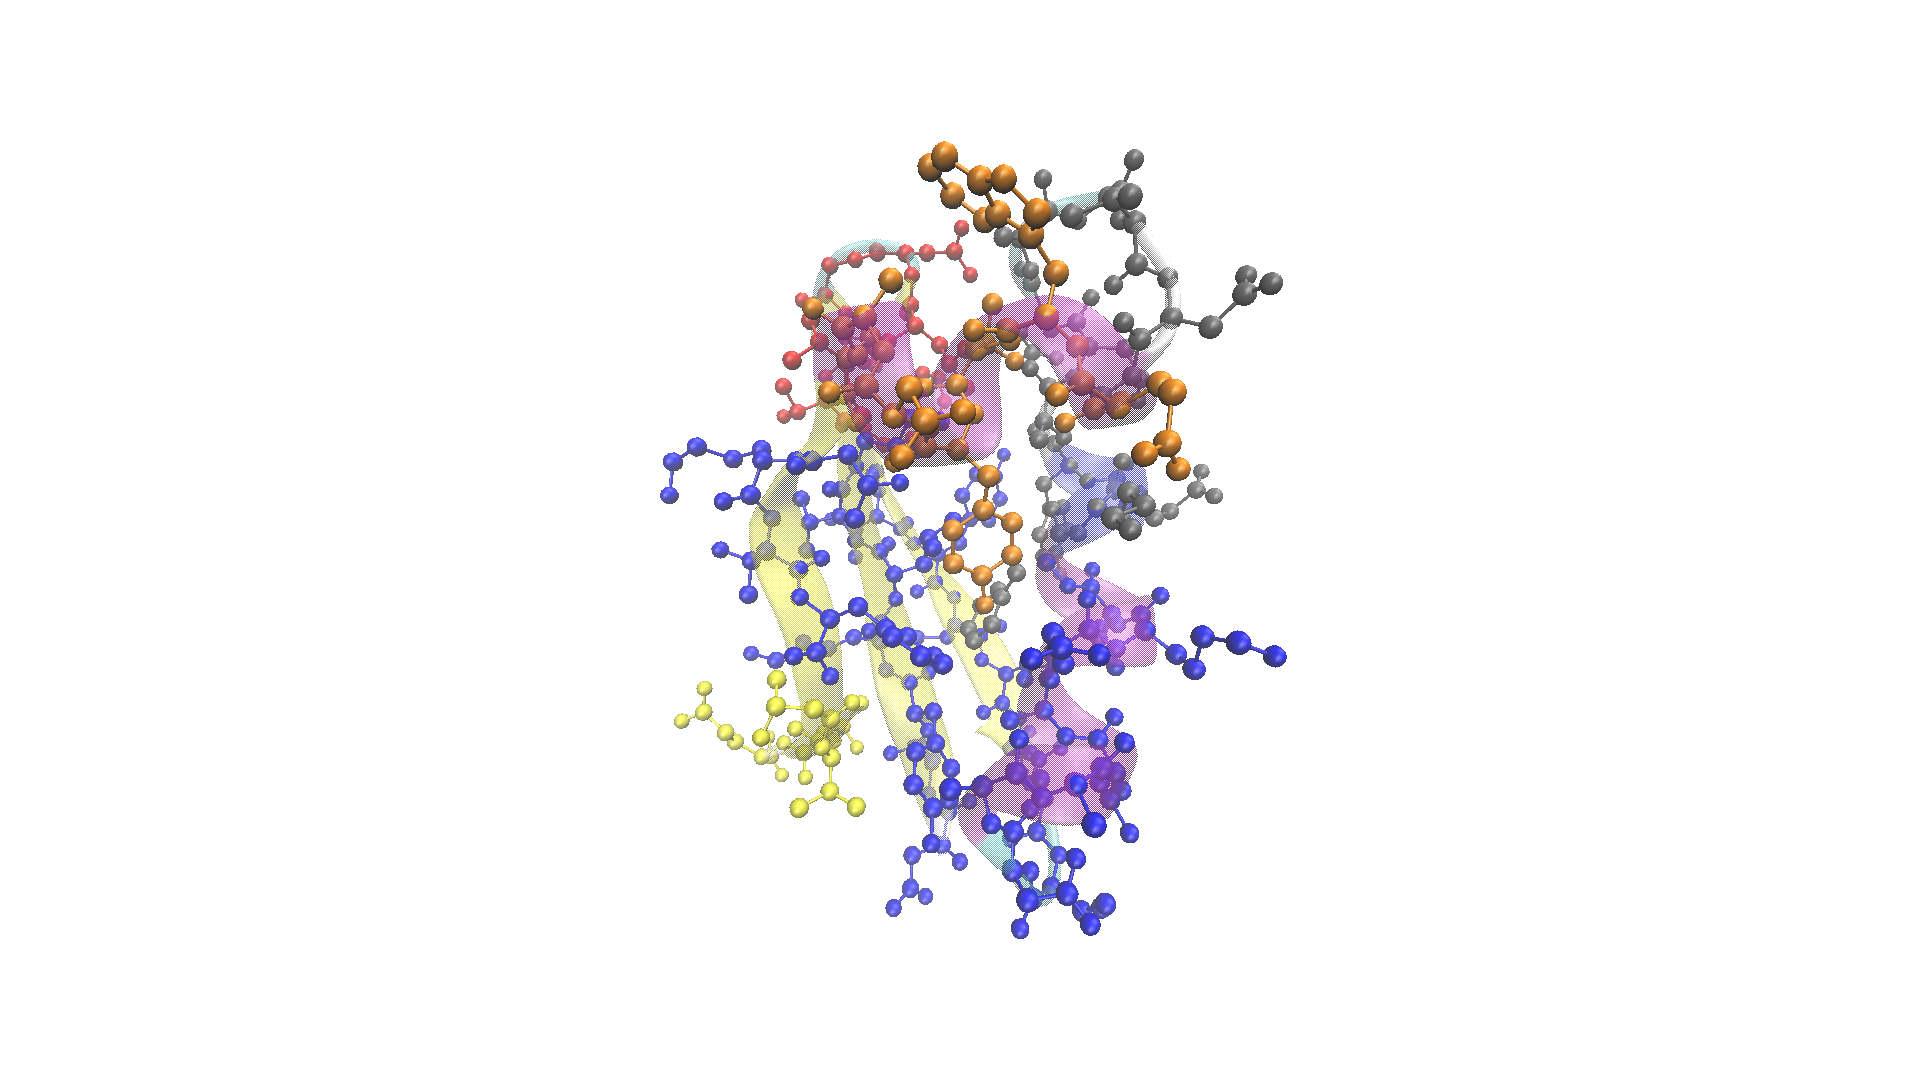
\includegraphics[width=0.3\textwidth, trim={14.815cm 0cm 14.815cm 0cm},clip]{NuG2_state_1.png}
  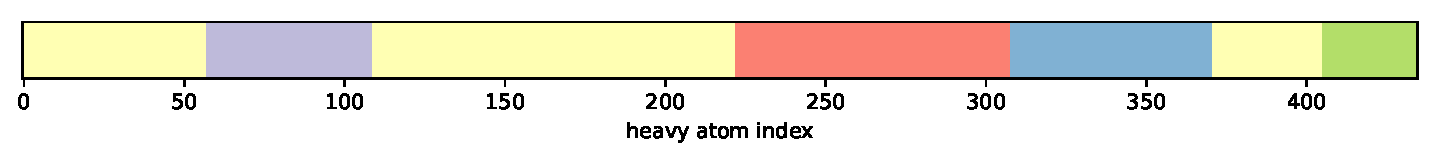
\includegraphics[width=0.7\textwidth]{NuG2_clustering_result_state_2.pdf}}\\
  \subfloat[Metastable State 3]{
  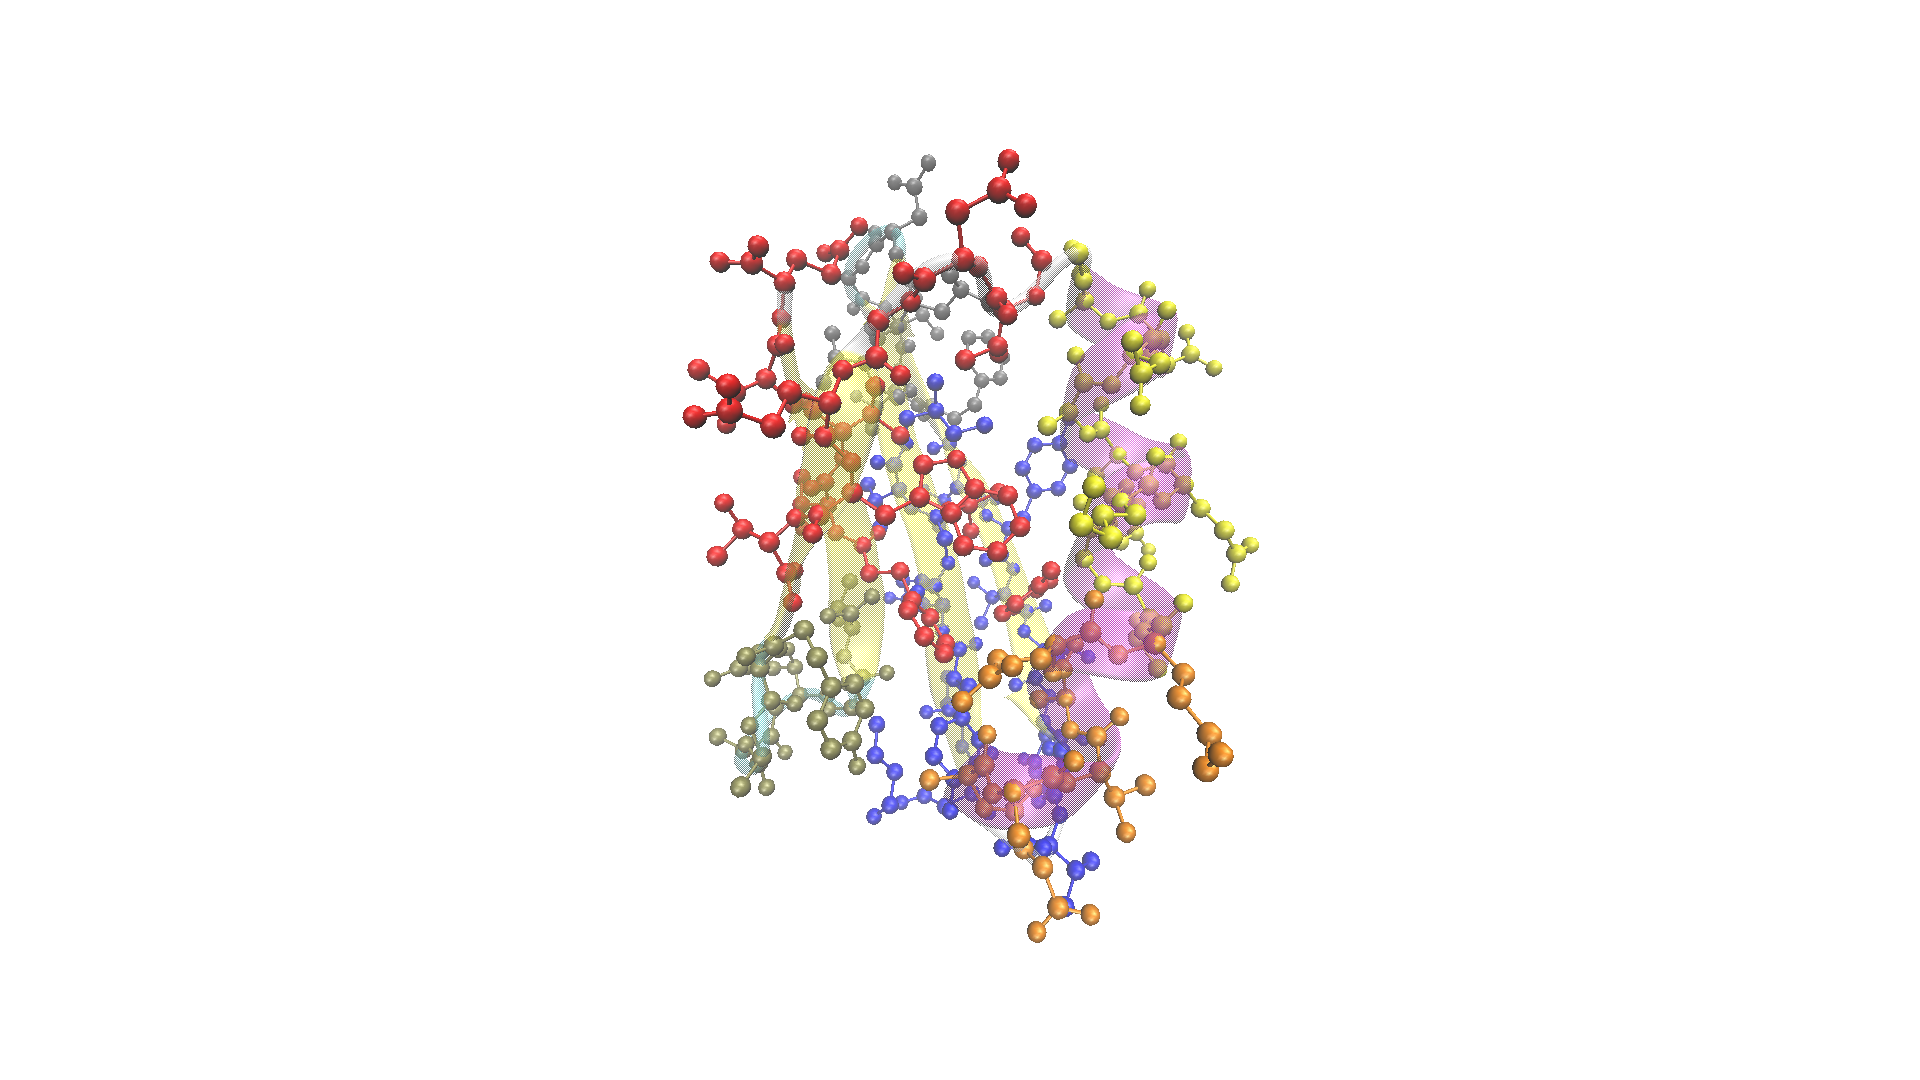
\includegraphics[width=0.3\textwidth, trim={14.815cm 0cm 14.815cm 0cm},clip]{NuG2_state_2.png}
  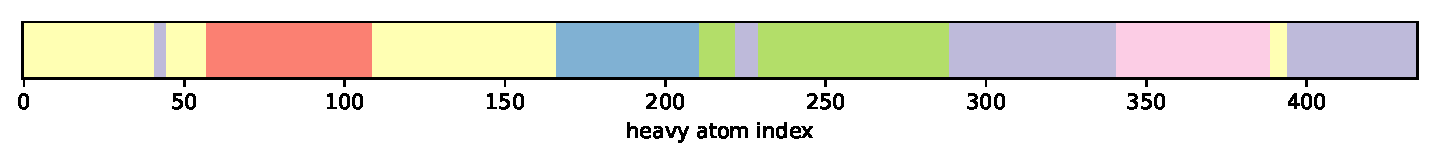
\includegraphics[width=0.7\textwidth]{NuG2_clustering_result_state_3.pdf}}\\
  \caption{\label{NuG2}Coherent domains for each metastable state of Protein G. Three metastable states are identified. For state 1 and 2, five coherent domains are obtained; for state 3, there are six.}
\end{figure}

\clearpage

\subsection*{$\alpha$3D}

\begin{figure}[htbp]
  \centering
  \subfloat[Metastable State 1]{
  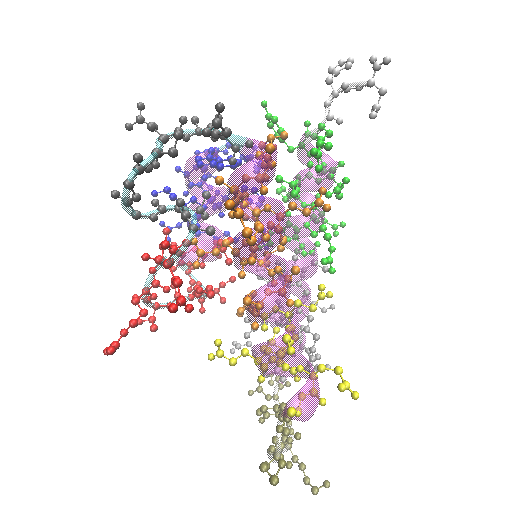
\includegraphics[width=0.3\textwidth, trim={0cm 0cm 0cm 0cm},clip]{A3D_state_0.png}
  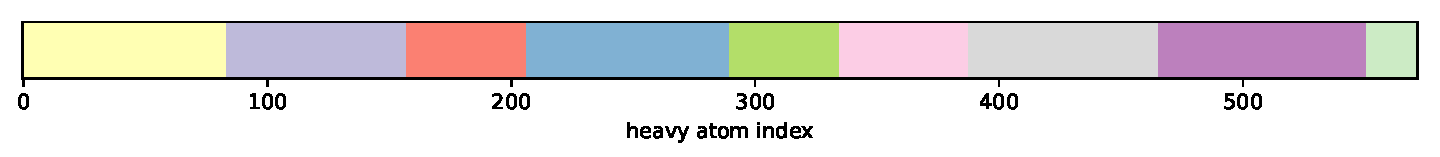
\includegraphics[width=0.7\textwidth]{A3D_clustering_result_state_1.pdf}}\\
  \subfloat[Metastable State 2]{
  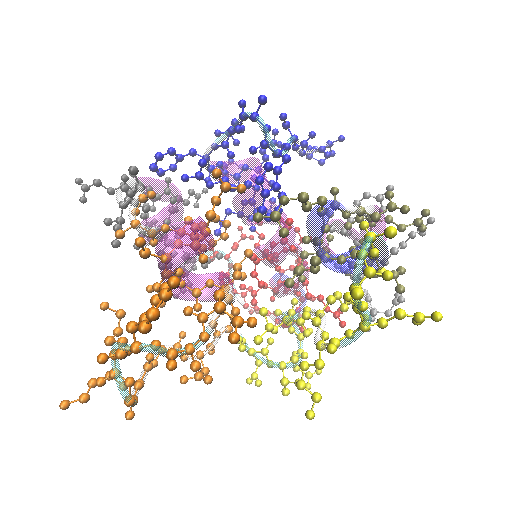
\includegraphics[width=0.3\textwidth, trim={0cm 0cm 0cm 0cm},clip]{A3D_state_1.png}
  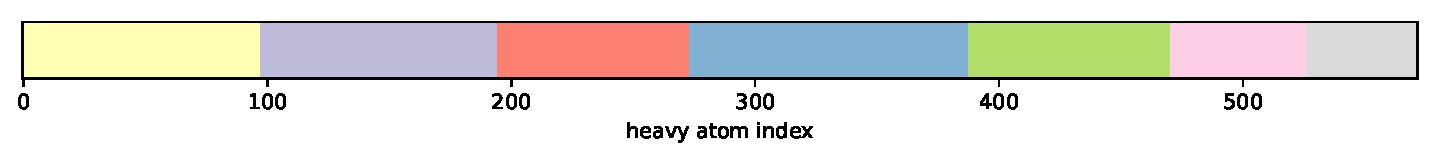
\includegraphics[width=0.7\textwidth]{A3D_clustering_result_state_2.pdf}}\\
  \subfloat[Metastable State 3]{
  \includegraphics[width=0.3\textwidth, trim={0cm 0cm 0cm 0cm},clip]{A3D_state_2.png}
  \includegraphics[width=0.7\textwidth]{A3D_clustering_result_state_3.pdf}}\\
\end{figure}

%\addtocounter{figure}{-1}

\begin{figure}[htbp]
  \addtocounter{subfigure}{3}
  \subfloat[Metastable State 4]{
  \includegraphics[width=0.3\textwidth, trim={0cm 0cm 0cm 0cm},clip]{A3D_state_3.png}
  \includegraphics[width=0.7\textwidth]{A3D_clustering_result_state_4.pdf}}\\
  \subfloat[Metastable State 5]{
  \includegraphics[width=0.3\textwidth, trim={0cm 0cm 0cm 0cm},clip]{A3D_state_4.png}
  \includegraphics[width=0.7\textwidth]{A3D_clustering_result_state_5.pdf}}\\
  \caption{\label{A3D}Coherent domains for each metastable state of $\alpha$3D. Five metastable states are identified. For state 1 and 4, nine coherent domains are obtained; for state 2 an 3, there are seven; eight coherent domains are obtained for state 5.}
\end{figure}

\clearpage

\subsection*{$\lambda$-repressor}

\begin{figure}[htbp]
  \centering
  \subfloat[Metastable State 1]{
  \includegraphics[width=0.3\textwidth, trim={0cm 0cm 0cm 0cm},clip]{lambda_state_0.png}
  \includegraphics[width=0.7\textwidth]{lambda_clustering_result_state_1.pdf}}\\
  \subfloat[Metastable State 2]{
  \includegraphics[width=0.3\textwidth, trim={0cm 0cm 0cm 0cm},clip]{lambda_state_1.png}
  \includegraphics[width=0.7\textwidth]{lambda_clustering_result_state_2.pdf}}\\
  \subfloat[Metastable State 3]{
  \includegraphics[width=0.3\textwidth, trim={0cm 0cm 0cm 0cm},clip]{lambda_state_2.png}
  \includegraphics[width=0.7\textwidth]{lambda_clustering_result_state_3.pdf}}\\
\end{figure}

%\addtocounter{figure}{-1}

\begin{figure}[htbp]
  \addtocounter{subfigure}{3}
  \subfloat[Metastable State 4]{
  \includegraphics[width=0.3\textwidth, trim={0cm 0cm 0cm 0cm},clip]{lambda_state_3.png}
  \includegraphics[width=0.7\textwidth]{lambda_clustering_result_state_4.pdf}}\\
  \caption{\label{lambda}Coherent domains for each metastable state of $\lambda$-repressor. Four metastable states are identified. For state 1 and 3, six coherent domains are obtained; for state 2 and 4, there are five.}
\end{figure}

\clearpage

\section*{Coherent Domains of Each Simulation for 2 Intrinsically Disordered Proteins}

Similar to the fast-folding proteins, in this section, we provide the details of the coherent domains of simulations under different conditions for the 2 intrinsically disordered proteins. We show the representative structure of the protein under each condition on the left, and plot the definition of coherent domains linearly along the heavy atom sequence on the right in different colors. The simulation details of ACTR can be found in reference \cite{ACTR}, and MYC in reference \cite{MYC}.

\subsection*{ACTR}

\begin{figure}[htbp]
  \centering
  \subfloat[Urea 0M]{
  \includegraphics[width=0.3\textwidth, trim={7cm 0cm 7cm 0cm},clip]{ACTR_traj_1.png}
  \includegraphics[width=0.7\textwidth]{ACTR_clustering_result_traj_1.pdf}}\\
  \subfloat[Urea 1M]{
  \includegraphics[width=0.3\textwidth, trim={7cm 0cm 7cm 0cm},clip]{ACTR_traj_2.png}
  \includegraphics[width=0.7\textwidth]{ACTR_clustering_result_traj_2.pdf}}\\
  \subfloat[Urea 2.5M]{
  \includegraphics[width=0.3\textwidth, trim={7cm 0cm 7cm 0cm},clip]{ACTR_traj_3.png}
  \includegraphics[width=0.7\textwidth]{ACTR_clustering_result_traj_3.pdf}}\\
\end{figure}

%\addtocounter{figure}{-1}

\begin{figure}[htbp]
  \addtocounter{subfigure}{3}
  \subfloat[Urea 5M]{
  \includegraphics[width=0.3\textwidth, trim={7cm 0cm 7cm 0cm},clip]{ACTR_traj_4.png}
  \includegraphics[width=0.7\textwidth]{ACTR_clustering_result_traj_4.pdf}}\\
  \subfloat[Urea 7M]{
  \includegraphics[width=0.3\textwidth, trim={7cm 0cm 7cm 0cm},clip]{ACTR_traj_5.png}
  \includegraphics[width=0.7\textwidth]{ACTR_clustering_result_traj_5.pdf}}\\
  \subfloat[Urea 9M]{
  \includegraphics[width=0.3\textwidth, trim={7cm 0cm 7cm 0cm},clip]{ACTR_traj_6.png}
  \includegraphics[width=0.7\textwidth]{ACTR_clustering_result_traj_6.pdf}}\\
  \caption{\label{ACTR}Coherent domains for each simulation of ACTR. For the simulation under 0M urea, three coherent domains are obtained; for the simulations under 1M and 9M urea, there are four; for the simulations under 2.5M and 7M urea, there are five; six coherent domains are obtained for the simulation under 5M urea.}
\end{figure}

\clearpage

\subsection*{MYC}

\begin{figure}[htbp]
  \centering
  \subfloat[NaCl 0.1M]{
  \includegraphics[width=0.3\textwidth, trim={32cm 0cm 32cm 0cm},clip]{MYC_traj_1.png}
  \includegraphics[width=0.7\textwidth]{MYC_clustering_result_traj_1.pdf}}\\
  \subfloat[NaCl 0.5M]{
  \includegraphics[width=0.3\textwidth, trim={32cm 0cm 32cm 0cm},clip]{MYC_traj_2.png}
  \includegraphics[width=0.7\textwidth]{MYC_clustering_result_traj_2.pdf}}\\
  \subfloat[NaCl 1.0M]{
  \includegraphics[width=0.3\textwidth, trim={32cm 0cm 32cm 0cm},clip]{MYC_traj_3.png}
  \includegraphics[width=0.7\textwidth]{MYC_clustering_result_traj_3.pdf}}\\
\end{figure}

\clearpage

\begin{figure}
  \addtocounter{subfigure}{3}
  \subfloat[NaCl 2.0M]{
  \includegraphics[width=0.3\textwidth, trim={32cm 0cm 32cm 0cm},clip]{MYC_traj_4.png}
  \includegraphics[width=0.7\textwidth]{MYC_clustering_result_traj_4.pdf}}\\
  \caption{\label{MYC}Coherent domains for each simulation of MYC. For the simulations under 0.1M, 0.5M and 2.0M NaCl, four coherent domains are obtained; for the simulation under 1.0M NaCl, there are six.}
\end{figure}

\bibliography{bib}

\bibliographystyle{Science}

\end{document}